\chapter{Development of a Web-Based Visualization Tool for the Comparison of 
Organism Genome Properties} \label{micromeda-client}

As discussed in Chapter \ref{introduction}, a client web application provides 
Micromeda's \gls{ui}. This client's role is to provide users with a streamlined 
interface for visualizing patterns of property and step assignment found across 
organisms. These assignment data are provided to the client in the form of a 
user-uploaded Micromeda file (Section \ref{MicromedaFiles}). After upload, these 
files are sent to Micromeda-Server (Chapter \ref{micromeda-server}) where they 
are parsed and used to provide data to the client. The client can request these 
data through a series of web \gls{api} endpoints (Section \ref{endpoints}) 
provided by Micromeda-Server. This chapter discusses the client web application, 
called Micromeda-Client, in detail. Links to a demonstration of the client 
interface can be found in Section \ref{client-demo}. Source code for Micromeda-Client is 
located at 
\href{https://github.com/Micromeda/micromeda-client}{github.com/Micromeda/micromeda-client}.

\section{Visualisation Design} \label{visualization-design}

One of the core uses of Genome Properties assignment data is to mine it for 
biologically relevant patterns in the presence and absence of biochemical 
pathways or structural features across organisms. One of the best ways to detect 
such patterns is through the use of data visualization. By visualizing Genome 
Properties assignment data, users can make comparisons between organisms, 
pathways, and steps. Several example comparisons and their research relevance 
are listed below and are displayed in Fig. \ref{fig:client-analysis-types}. 

\begin{itemize}
\item By looking at the assignments of a single property across organisms, users 
can select subsets of organisms that may possess a specific phenotype (Fig. 
\ref{fig:client-analysis-types}a). Such comparisons are useful in scientific 
fields where specific traits must be identified. Such fields include pathogen 
research, microbial ecology, bioengineering and bioprocess engineering, among 
others.
\item By comparing the assignments of multiple genome properties, users can 
identify patterns of conservation across organisms in a dataset (Fig. 
\ref{fig:client-analysis-types}c). In microbial ecology, such comparisons can be 
used to identify microorganisms that fit specific biochemically determined 
ecological niches (\textit{e}.\textit{g}., photoferrotrophy).
\item By looking at the step assignments of a single property of a single 
organism, users can evaluate the correctness of a property assignment (Fig. 
\ref{fig:client-analysis-types}b). A property might be assigned NO or PARTIAL 
because it is missing only a few required steps; However, it may possess many 
other steps that are not required (Fig. \ref{fig:client-analysis-types}b). Being 
able to look at all step assignments for the property would allow users to 
determine why a property has been given a specific assignment.
\item By comparing step assignments of single property across multiple 
organisms, users can see whether pathway steps are retained across organisms 
(Fig. \ref{fig:client-analysis-types}d). If a property step is not retained in a 
large assortment of phylogenetically distant genomes, it may not be required by 
a pathway or may be carried out by proteins that are non-canonical (Fig. 
\ref{fig:client-analysis-types}d). Such non-canonical proteins may not possess 
domains used by Genome Properties but nonetheless do still carry out a missing 
pathway step.
\end{itemize}

\begin{figure}[!ht]
  \centering
	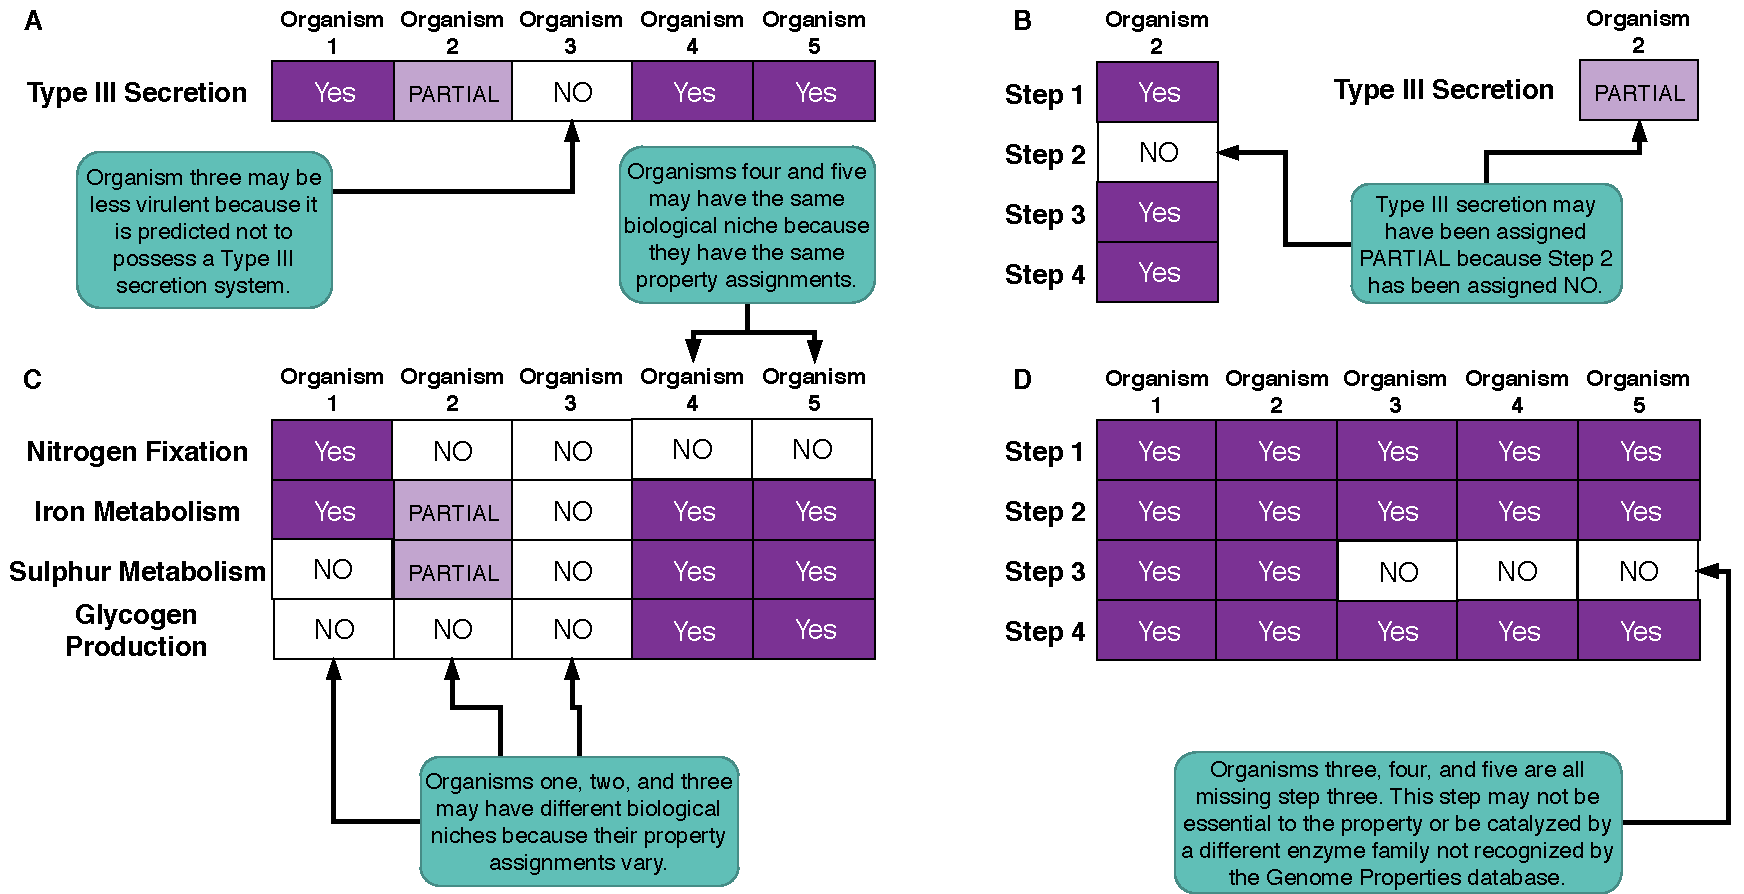
\includegraphics[width=\textwidth]{media/analysis_types.pdf}
	 \caption[Examples of different pathway analysis tasks that can be supported by 
the visualization of Genome Properties data.]{\textbf{Examples of different 
pathway analysis tasks that can be supported by the visualization of Genome 
Properties data.} Comparisons can be made between 
organisms, pathways, or pathway steps.}
	 \label{fig:client-analysis-types}
\end{figure}

If Micromeda-Client is to support these listed comparisons, the data visualization 
method used must allow users to perform the following tasks.

\begin{itemize}
\item Track assignments across organisms
\item Assess the magnitude of assignments
\item Aggregate assignments into summaries
\item Explore how these aggregate summaries are derived
\item Find assignments of interest
\end{itemize}

When a visualization approach was selected for use by Micromeda-Client, the 
compatibility of the visualization with these tasks was prioritized.

\subsection{An Overview of Genome Properties Data}

Specific visualization techniques are better suited for presenting certain types 
of the data over others, and it is essential first to discuss the nature of data to 
be visualized before discussing how a specific visualization approach was 
selected for Micromeda-Client. At its core, the data presented by 
Micromeda-Client consist of assignments for genome properties and their steps. 
Such assignments are ordinal data 
\cite{richardson2018genome,agresti2010analysis}, as their states of YES, 
PARTIAL, and NO are ordered. It should be noted that properties are connected 
hierarchically \cite{richardson2018genome} and thus this structure is 
hierarchical data \cite{richardson2018genome,samet1990applications}. The 
property hierarchy influences the ordinal assignment data of each property 
because assignments of parent genome properties can be used to summarize the 
assignments of child genome properties or steps \cite{richardson2018genome}. 
Each piece of assignment data that is presented by Micromeda-Client also belongs 
to a specific property or step and organism. Thus, the Genome Properties data 
can also be considered to be multidimensional 
\cite{pedersen1999multidimensional}.

\subsection{How Micromeda-Client Visualizes Assignment Data}
\label{client-visualization}

When designing a data visualization, often specific visualization techniques 
present themselves intuitively as potential candidates, and this was the case 
while designing Micromeda-Client. An appropriate visualization for 
multidimensional datasets, such as Genome Properties assignments, is a heat map 
\cite{wilkinson2009history,tufte2001visual}(Fig. 
\ref{fig:client-analysis-types}) and this visualization technique was the one 
chosen for the client (Fig. \ref{fig:client-analysis-types}). A heat map was 
chosen over the competing visualization techniques such as bubble charts 
\cite{tufte2001visual}, circular maps 
\cite{ward2002taxonomy,stothard2004circular}, or treemaps 
\cite{shneiderman1998tree} due to the number of variables that needed to be 
plotted by the client and the superior space utilization of heat maps, which 
mimic the square dimensions of the computer monitors they are displayed on 
\cite{muramalla2017radial}.

Micromeda-Client's heat map uses cell position to indicate what assignment 
belongs to what property or step and organism (Fig. 
\ref{fig:client-analysis-types}). Because most Micromeda files contain 
information about fewer organisms than there are properties in the Genome 
Properties database (\textit{e}.\textit{g}., approximately 40 organisms versus 
1296 properties), assignments for the same property, but from different 
organisms, are positioned within the same heat map row (\textit{i}.\textit{e}, 
property labels are placed along y-axis rather the x-axis of the heat map). 
Columns are used to group assignments from the same organism across properties 
or steps. This configuration leads to a heat map that is much taller than it is 
wide and requires that users scroll vertically. Vertical scrolling is much more 
convenient than scrolling horizontally because it allows users to scroll the 
visualization quickly by using their mouse.

The magnitude of each assignment is encoded using cell colour (Fig. 
\ref{fig:client-analysis-types}). Because assignments are ordinal data, it makes 
sense to encode assignments using colour saturation, rather than hue 
\cite{munzner2015visualization}. For the heat map, a purple cell colour scheme 
was chosen to ensure that the diagram is interpretable by those with colour 
blindness. Specifically, colours were optimized for users with severe 
deuteranopia (\textit{i}.\textit{e}., complete loss of green cones), which, though rarer, has 
stronger Red-green colour blindness affects (see 
\href{http://wikipedia.org/wiki/Color_blindness#Classification}{wikipedia.org/wiki/Color\_blindness\#Classification}). 
A web service called ColorBrewer 
(\href{http://colorbrewer2.org}{colorbrewer2.org}) was used to select cell 
colours, and a tool called Sim Daltonism 
(\href{http://github.com/michelf/sim-daltonism}{github. 
com/michelf/sim-daltonism}) was used to ensure colour blind compatibility of the 
entire diagram. 

Any visualization technique used is also challenged by the magnitude of data to 
be presented by Micromeda-Client. For example, if the heat map described at the 
top of this section displayed all assignments for only a few organisms, then its 
size would prevent users from finding or tracking assignments quickly across 
organisms. As of version 2.0 of the Genome Properties database, there are 1296 
properties and 6525 steps \cite{richardson2018genome}. If the client were used 
to generate a single heat map representing the assignments of all properties, 
with each cell being 5 mm tall, then the heat map produced would be 
approximately 6.5 meters tall (\textit{i}.\textit{e}., fifteen vertical pages on 
a 24" monitor). If a similar heat map was made, but for assignments of all 
property steps, then the heat map generated would be over 32.6 meters tall 
(\textit{i}.\textit{e}., seventy-five vertical pages on a 24" monitor). If both 
of these heat maps were combined, then the resulting heat map would be even 
longer. Micromeda-Client's visualization interface addresses the length issue by 
using interactive aggregation and disaggregation \cite{munzner2015visualization} 
of assignment rows to reduce the overall length of the client's assignment heat 
map (Fig. \ref{fig:visualization-philosophy}). This reduced length facilitates 
rapid visual exploration of property and step assignments.

Micromeda-Client's \gls{ui} allows users to manipulate the contents of the 
client's assignment heat map to show and hide properties and steps according to 
their position in the Genome Properties \gls{dag} \cite{richardson2018genome} 
(Fig. \ref{fig:visualization-philosophy}). Because the Genome Properties 
\gls{dag} arranges individual properties hierarchically, the assignments of 
properties closer to the root can be used to summarize the assignments of 
properties closer to the \gls{dag}'s leaves (Fig. 
\ref{fig:visualization-philosophy}). In the context of a heat map, this 
hierarchical assignment summarization means that a row of assignments for a 
parent property can be used to summarize the rows of assignments of this 
property's children, either other properties or steps 
(Fig.\ref{fig:visualization-philosophy} and Fig. 
\ref{fig:client-analysis-types}). Micromeda-Client provides mechanisms to expand 
and collapse heat map rows to display either parent summary assignments or more 
detailed child assignments (Fig. \ref{fig:visualization-philosophy}).

\begin{figure}[!ht]
  \centering
	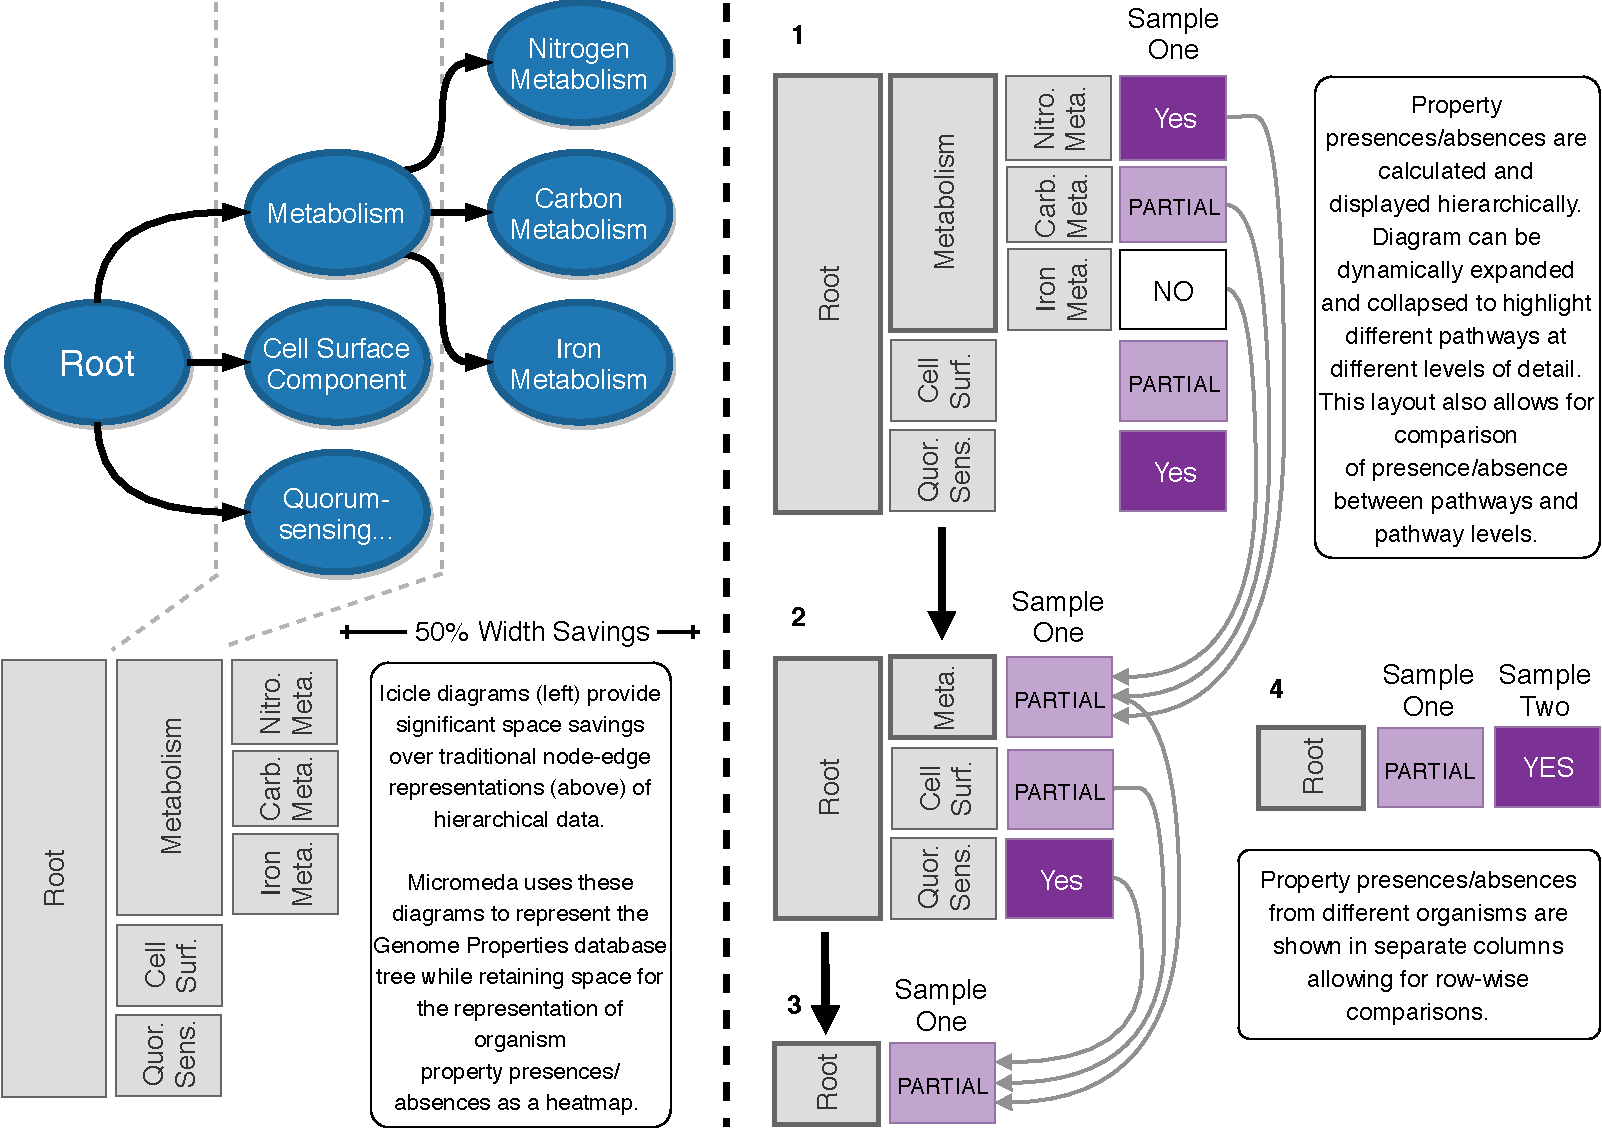
\includegraphics[width=0.8\textwidth]{media/visualization_design_philosphy.pdf}
	 \caption[Overview of the components of Micromeda's visualization design that 
are critical to user interactivity.]{\textbf{Overview of the components of 
Micromeda's visualization design that are critical to user interactivity.} The 
use of an icicle diagram allows the final visualization to be more compact. 
Clicking nodes in the icicle diagram changes the shape of the heat map by adding 
and removing rows.}
	 \label{fig:visualization-philosophy}
\end{figure}

One critical design decision for Micromeda-Client was how to let users control 
the aggregation and disaggregation of heat map rows. To support this 
usage, a new visualization component to Micromeda-Client was designed, in 
addition to the assignment heat map. Specifically, the client uses a horizontal 
icicle diagram\footnote{Traditional icicle diagrams have leaf nodes facing 
downwards. The icicle diagram used by Micromeda-Client is rotated 90 degrees and 
has its leaf nodes facing to the right.} placed left of the heat map. Icicle 
diagrams were chosen over other ways of visualizing hierarchical data, such as 
trees, due to their spacial compactness (Fig. 
\ref{fig:visualization-philosophy}). The icicle diagram is used to control the 
heat map's content (Fig. \ref{fig:visualization-philosophy}). Icicle diagrams 
are used to display hierarchical data, such as the parent-child relationship 
between properties and between properties and their steps. With the 
Micromeda-Client, each genome property and step in the Genome Properties 
database is assigned a node in the icicle diagram (Fig. 
\ref{fig:visualization-philosophy}). Nodes that represent properties are 
labelled gray and nodes that represent steps of leaf properties are labelled 
green. The leaf nodes of the icicle diagram are aligned to rows in the adjacent 
heat map (Fig. \ref{fig:visualization-philosophy}) that contain the assignments 
for the property or step that the node represents.

With Micromeda-Client, the nodes in the icicle diagram are given a state of 
either on or off. When a user clicks a node in an off state, a new column is 
added to the icicle diagram. This column's contents includes new icicle nodes 
representing the clicked node's children. Simultaneously, new assignment rows 
are added to the heat map. These rows belong to the same properties or steps 
that the newly added icicle diagram nodes represent. The new heat map rows 
replace the clicked node's assignment row. The new icicle nodes and heat map 
rows are vertically aligned. Each new node in the icicle diagram has the same 
height as its parent. The clicked node's shape is expanded vertically to align 
with the top and bottom of its first and last child node cells, respectively. 
The overall length of the icicle diagram and heat map is extended. If the user 
clicks the previous clicked node once again, then the expansion process 
is reversed. The child nodes and their assignment rows are removed from the 
visualization (Fig. \ref{fig:visualization-philosophy}), the clicked cell 
returns to its original shape, and its matching summary assignment row is placed 
back into the heat map (Fig. \ref{fig:visualization-philosophy}). Child 
assignment rows are also removed from the heat map. Columns in the icicle 
diagram are deleted, upon child cell removal, only if all sibling or cousin 
nodes to the clicked node also have no children displayed.

The visualization strategy chosen for Micromeda-client supports the required 
tasks presented at the top of this section. The heat map allows users to track 
assignments across organisms and assess their magnitude. The interactive 
aggregation control provided by the icicle diagram allows users to aggregate 
step and property assignments into summaries. These aggregate assignments can 
later be disaggregated to show child assignments, allowing users to explore how 
the parent assignments were derived. As the icicle diagram follows the structure 
of the Genome Properties \gls{dag}, specific assignments can be found quickly by 
following the \gls{dag}'s structure from parent to child. Searching for 
properties is further enhanced by Micromeda-Client's ability to search for 
properties by name. This search functionality is discussed in the next section.

\section{Additional Features of Micromeda-Client's Interface} 
\label{client-additional-features}

In addition to the visualization capability presented in Section 
\ref{client-visualization}, the client's interface also possesses several other 
features that help users explore their data. In the top right corner of the 
\gls{ui} is a text-based search box (Fig. \ref{fig:micromeda-interface}). This 
box allows users to search for properties by entering a text string containing 
either a property name or identifier. As the user enters this string, a list of 
matching property names are displayed in a drop-down menu (Fig. 
\ref{fig:micromeda-interface}). As the user enters additional information, this 
list of possible matches shrinks. If the user clicks one of these property 
names, then the Micromeda-Client will automatically scroll to the heat map row 
where assignments for the clicked property are located. If the property is not 
shown in the current version of the heat map, then it will be added by 
disaggregating heat map rows in a path towards the property. This path is built 
recursively by disaggregating parent properties along a path from the root of 
the Genome Properties \gls{dag} to the property that was clicked in the search 
menu. As the client diagram scrolls, the X-axis labels remain in a fixed 
position to provide users with sample/genome name information for any assignment 
views. A similar scrolling behaviour as to when a search bar item is clicked is 
also activated when a user clicks a node in the icicle diagram. The diagram's 
X-axis is scrolled to align with the clicked node's associated heat map row.

\begin{figure}[!ht]
  \centering
	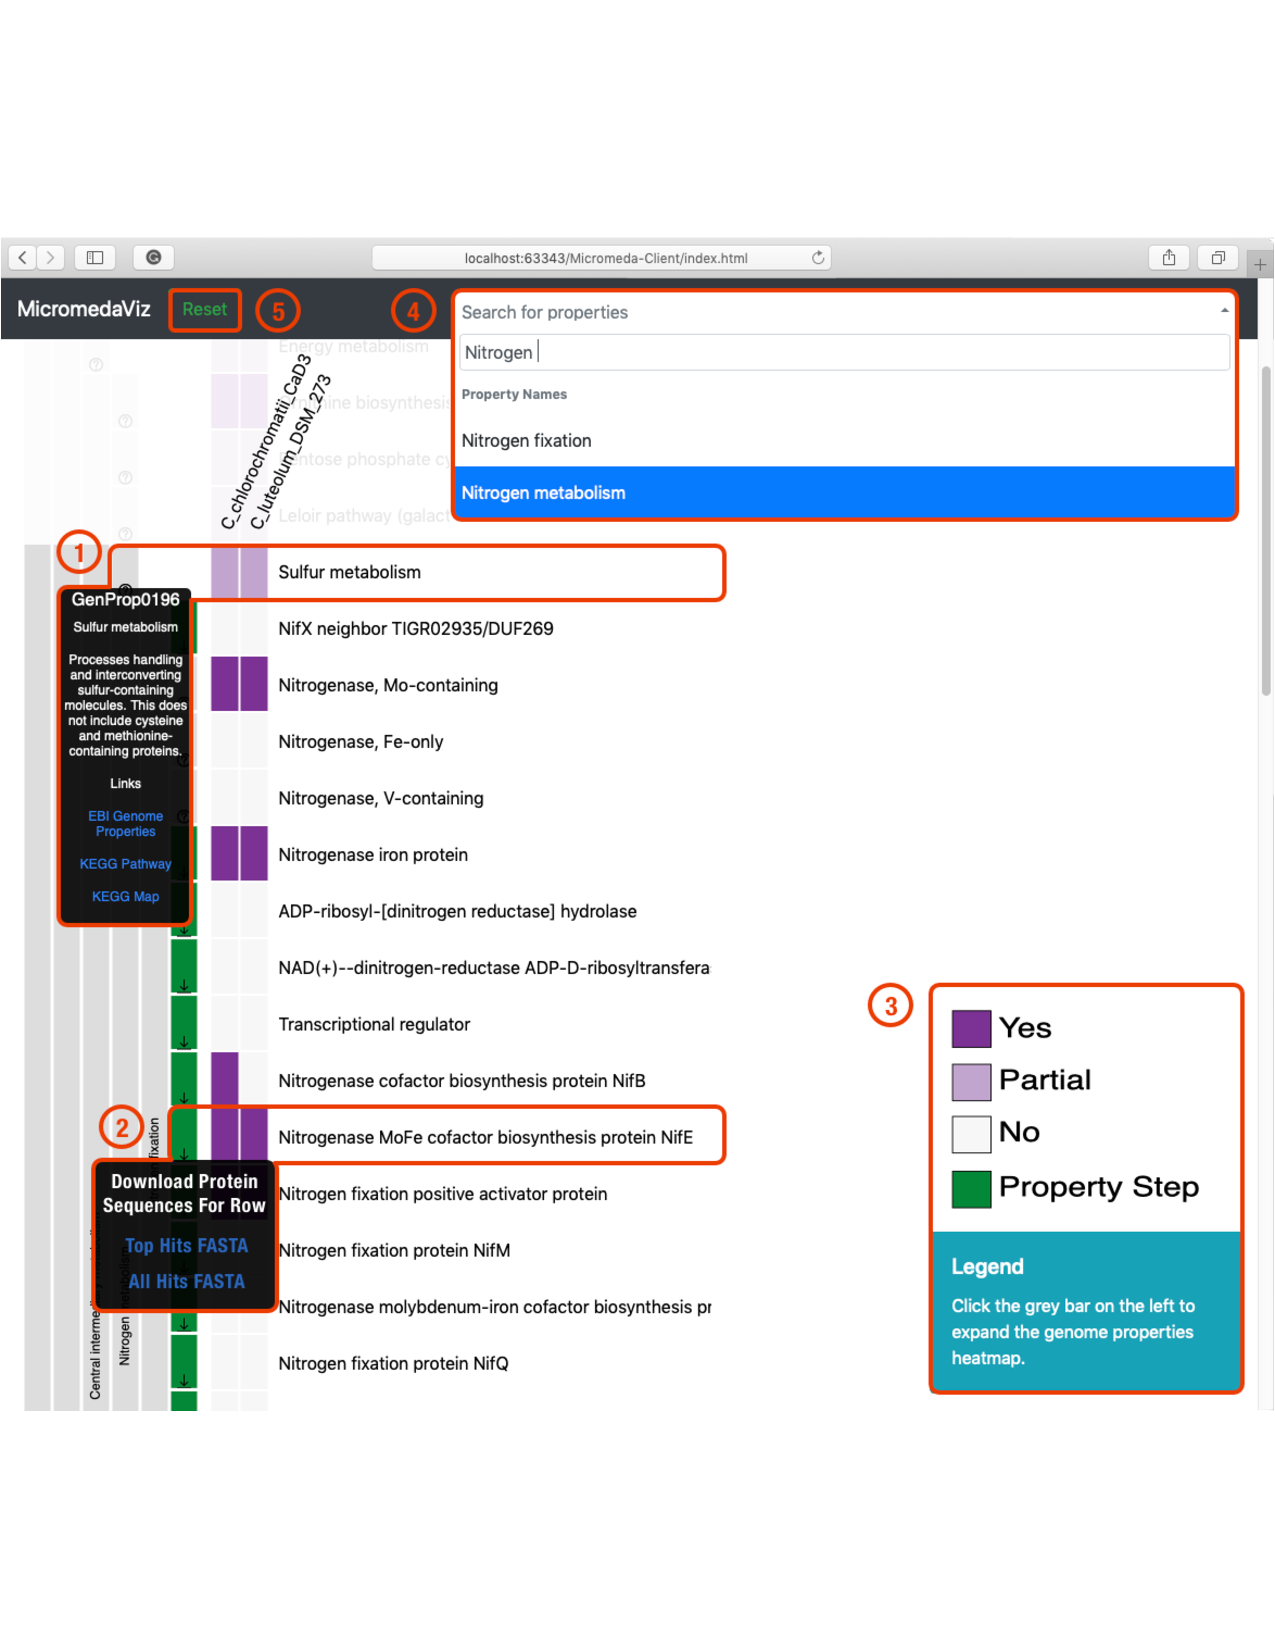
\includegraphics[width=0.9\textwidth]{media/micromeda-interface.pdf}
	 \caption[Web-browser window containing Micromeda’s heat map visualization and 
interface annotated to highlight the interface’s search and information 
gathering features.]{\textbf{Web-browser window containing Micromeda’s heat map 
visualization and interface annotated to highlight the interface’s search and 
information gathering features.} The interface provides functionality for getting 
additional information about properties and steps (1) and provides the ability 
to download protein sequences that support step assignments (2). A legend 
provides context to the heat map’s colour scheme (3). The interface also 
supports property searching (4) and possesses a reset button that allows users 
to reset the heat map to its initial loaded state (5).}
	 \label{fig:micromeda-interface}
\end{figure}

While users explore the heat map, it may be useful for them to be able to access 
more context about the displayed properties. The icicle diagram possesses 
question mark glyphs\footnote{A glyph is an elemental component of a data 
visualization. A data visualization is composed of a series of glyphs. Often 
glyphs are directly mapped to data points \cite{chen}.} at the bottom of each 
property node that facilitates access to an additional set of property 
information (Fig. \ref{fig:micromeda-interface}). When a user places their 
cursor over one of these glyphs, a pop-up box appears displaying information 
about the property that the glyph's node represents (Fig. 
\ref{fig:micromeda-interface}). When a user places their cursor over one of 
these glyphs, a pop-up box appears displaying information about the property 
that the glyph's node represents (Fig. \ref{fig:micromeda-interface}). This 
pop-up box includes the name of the property, a description of it, a link to the 
property on the \gls{ebi}  Genome Properties website (\textit{e}.\textit{g}., 
\href{https://www.ebi.ac.uk/interpro/genomeproperties/#GenProp0867}{ebi.ac.uk/interpro/genomeproperties/ 
\#GenProp0867}), and a list of links to equivalent records in other pathway 
databases such as \gls{kegg} \cite{kanehisa2000kegg} and MetaCyc 
\cite{karp2002metacyc}. The box is once again hidden when the user's cursor 
leaves the glyph or the pop-up box.

Some leaf property steps have a different glyph at the bottom of their nodes 
that is shaped like a download symbol (Fig. \ref{fig:micromeda-interface}). This 
glyph allows users to download protein sequences that support the existence of 
property steps. These download glyphs are only placed on nodes whose associated 
property steps are assigned YES in at least one organism displayed on the heat 
map. A pop-up box is also generated when these download glyphs are hovered over. 
This box contains two download links (Fig. \ref{fig:micromeda-interface}). The 
first link downloads a \gls{fasta} file containing the protein sequences that 
are most likely to carry out the step for each organism in a dataset\footnote{As 
discussed in the last paragraph of Section \ref{InterProDatabases}, each member 
database of the InterPro consortium possesses custom software that filters 
domain matches. These filtering tools implement rules, such as minimum match 
\gls{eval} scores or minimum alignment lengths, that remove false-positives. 
These rules are unique to each member database and are custom to the sequence 
search tool used by each database. InterProScan implements all sequence search 
tools and the false-positive filtering methods used by member databases. All 
domain matches identified by InterProScan are considered to be true positives, 
as they have passed scrutinous match filtering rules. Pygenprop utilizes these 
true-positive InterProScan matches to predict genome properties. For a given 
dataset, there are often multiple proteins with predicted true-positive domain 
matches that support a single genome property step. However, of this set 
matching proteins, the protein with the lowest match \gls{eval} score for the 
step’s supporting domain is most likely to carry out the step. As discussed in 
Subsection \ref{get-fasta-endpoint}, Micromeda-Server’s \textbf{get\_fasta} 
endpoint returns the \gls{fasta} formatted sequences of either all proteins 
containing a match to a domain that supports a property step, regardless of the 
organism, or a single protein per organism, each with the lowest \gls{eval} 
match to the domain that supports a property step. Micomeda-Client’s step 
protein download pop-up boxes provide web links that allow users to download 
\gls{fasta} files generated by the \textbf{get\_fasta} 
endpoint.\label{protein-download-note}}. The second link downloads a \gls{fasta} 
file containing any protein that could have carried out the step across all 
organisms in a dataset\textsuperscript{\ref{protein-download-note}}. When the 
cursor is removed from this download pop-up box or the glyph, then the pop-up 
box is hidden.

Micromeda-Client's interface also includes a reset button. This button resets 
the heat map and icicle diagram back to their starting configuration where only 
the top-level properties are shown (\textit{i}.\textit{e}., one level below the 
root of the Genome Properties \gls{dag}) to the user. Users can click this button 
to reset the diagram to allow them to search for other properties.

\section{Implementation} \label{client-implementation}

Micromeda-Client's interface consists of two web pages that were structured 
using \gls{html} \cite{HTML5}, styled using \gls{css} \cite{CSS3}, and scripted 
via \gls{javascript} \cite{flanagan2006javascript}. Users access one page for 
uploading user-generated Micromeda files, and another for presenting the 
visualizations of the file's data. To use Micromeda-Client, users must first 
navigate to the upload page and upload a Micromeda file. After the upload is 
complete, the user's browser will automatically redirect to the visualization 
page. Both pages are styled using the Bootstrap 3.0 \gls{css} framework 
\cite{spurlock2013bootstrap}. Bootstrap is used to set up page elements such as 
header navigation bars and drop-down menus. Bootstrap also makes each page 
compatible with tablet computers and phones as it will automatically restyle 
non-visualization page elements to fit on these smaller screens.

\section{Demonstration of the Client User Interface} \label{client-demo}

A demo of Micromeda’s client interface can be found at
\href{http://tundra-pear.glitch.me}{tundra-pear.glitch.me}. This demo is 
hosted in a way that certain features that require Micromeda-Server, such as 
Genome Property pop-ups and \gls{fasta} file downloads, are disabled. A video 
that displays these additional features can be found at
\href{https://tinyurl.com/wlgelmg}{tinyurl.com/wlgelmg}. 
This video also demonstrates the process of uploading a Micromeda file.

\subsection{Core Data Structures} \label{visual-data-structures}

The client visualization page uses two core data structures and they are both 
accessed during visualization generation. One is a diagram configuration array 
that contains a series of measurements. These measurements are used during 
diagram drawing and control spacing between heat map cells, heat map cell 
dimensions, the offset of axis labels, and other visualization details (Fig. 
\ref{fig:diagram-measurements}). The contents of this setting array are stored 
in a \gls{json} file \cite{bray2014rfc}, called 
\textbf{diagram\_configuration.json}, which is deployed alongside the \gls{html} 
files of the client. The second data structure is a copy of the Genome 
Properties \gls{dag} in the form of a tree (\textit{i}.\textit{e}., nodes with 
two parents are duplicated) of \gls{javascript} objects. Each of these objects 
represents a genome property or step and are linked together in parent-child 
relationships. This data structure is analogous to the one used by Pygenprop 
(Section \ref{GenomePropertiesTree-Class}). Each of these objects possesses an 
attribute, called assignments, containing a list of property assignments for the 
organism in a dataset. Micromeda-Client later uses these assignments during the 
generation of its heat map. These property and step objects also have an 
attribute, called \textbf{enabled}, containing a boolean 
(\textit{i}.\textit{e}., true or false). Elements of Micromeda's \gls{ui} 
manipulate the \textbf{enabled} attribute of objects in the property tree and 
this, in turn, manipulates the contents of the visualization (Fig. 
\ref{fig:tree-map-to-viz}). The \textbf{enabled} boolean of each property object 
tree determines whether the children of the property should be displayed in 
client visualization (Fig. \ref{fig:tree-map-to-viz}). The property tree is 
placed within a parent \gls{javascript} object. This property tree 
\gls{javascript} object is analogous to objects instantiated from Pygenprop's 
GenomePropertiesTree class (Section \ref{GenomePropertiesTree-Class}) and, as 
such, also possesses methods for property identifier-based lookups of the tree's 
underlying property objects and methods for extracting lists of the tree's root 
and leaf property objects.

\begin{figure}[!ht]
  \centering
	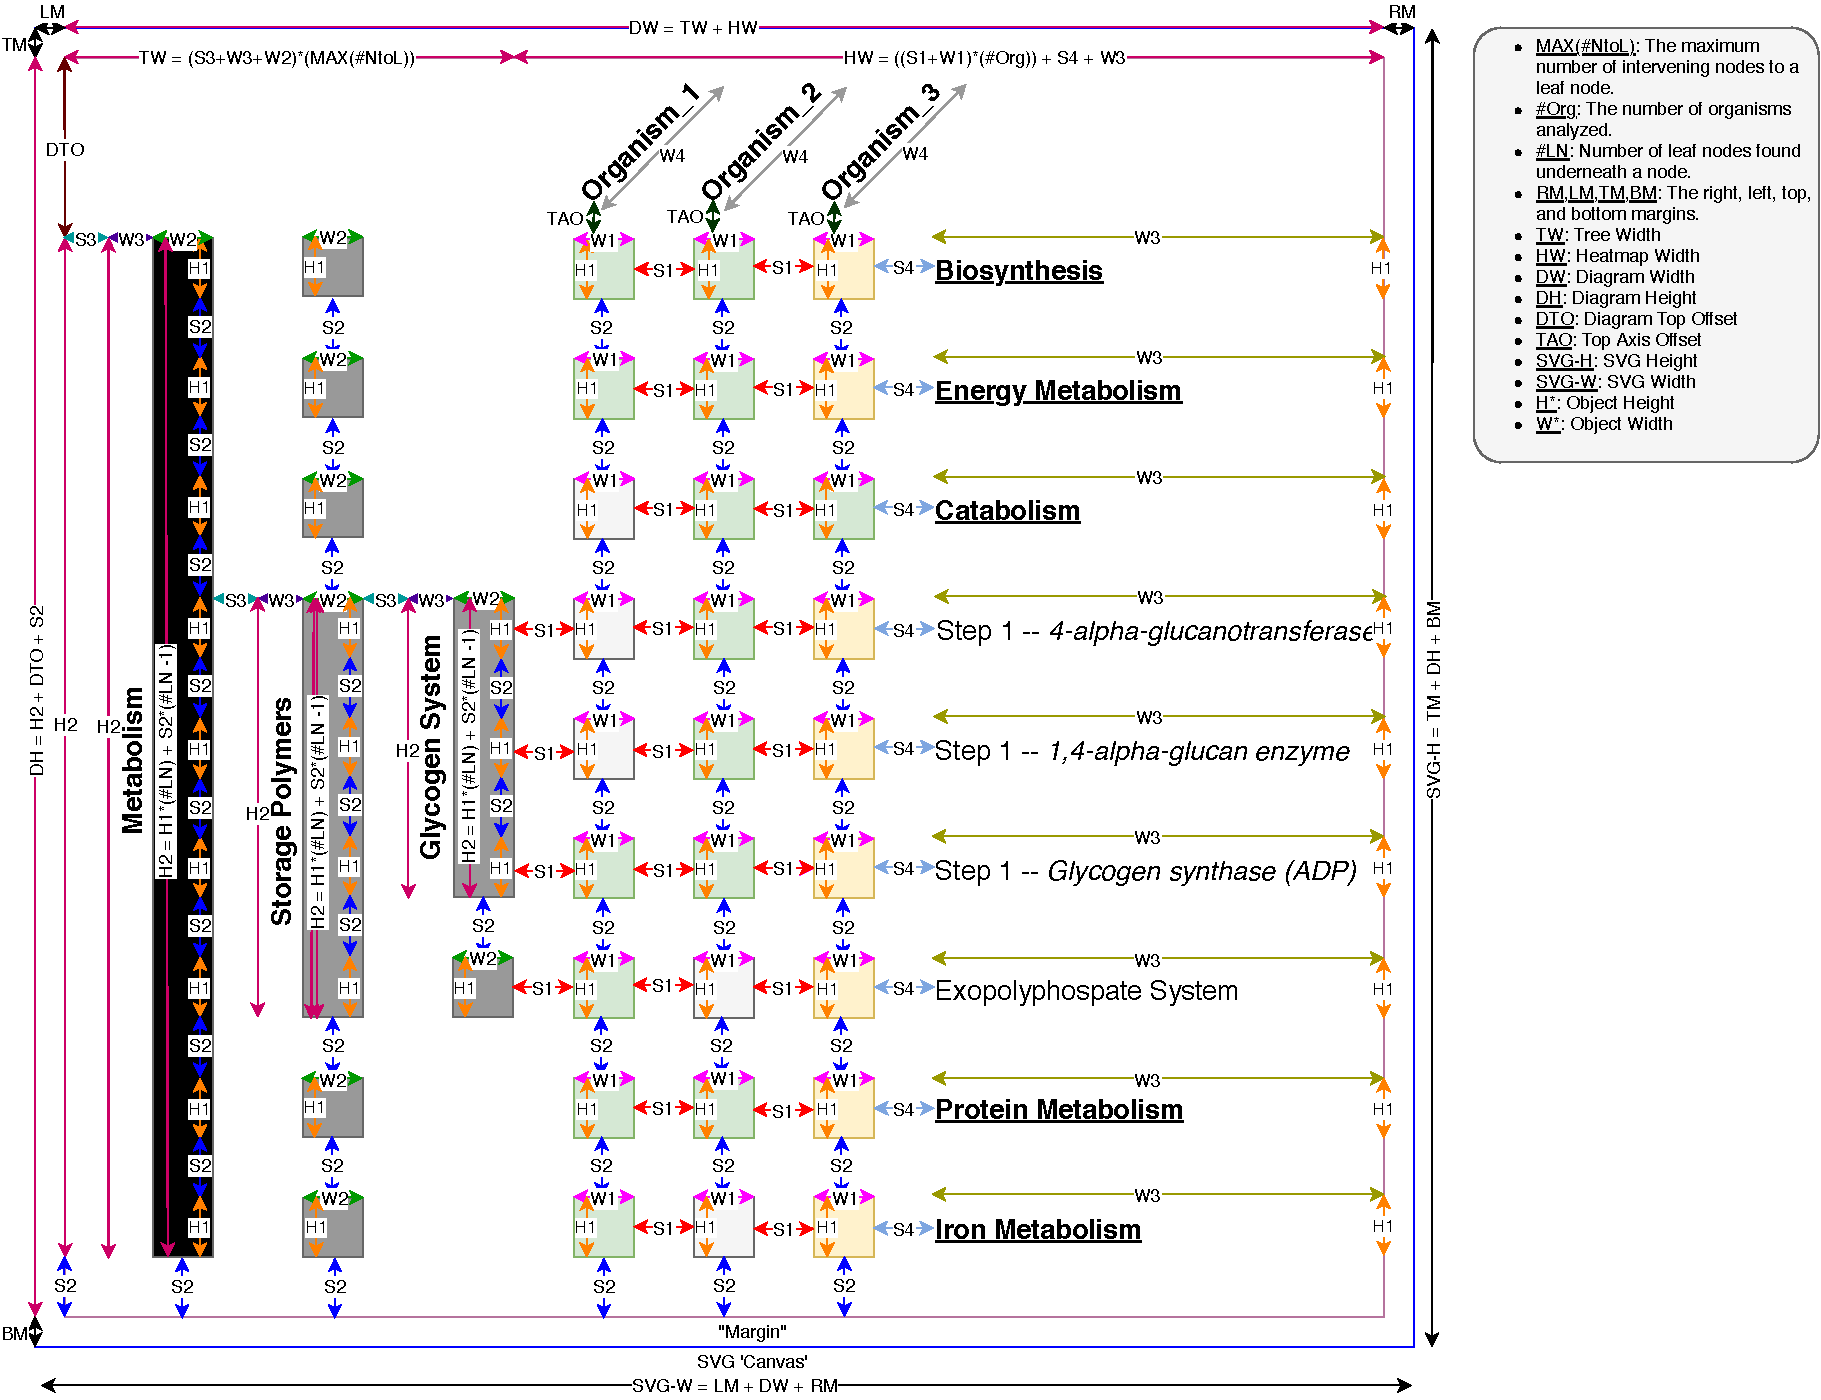
\includegraphics[width=\textwidth]{media/diagram_measurements.pdf}
	 \caption[How pre-defined spacing, width, and length values determine the 
layout of Micromeda-Client's diagrams.]{\textbf{How pre-defined spacing, width, 
and length values determine the layout of Micromeda-Client's diagrams.} Changes 
in these values can shift the size and spacing of the heat map's cells and axes. 
Dimension values are stored in an external file that is loaded upon diagram 
generation. The contents of this file can be modified to change the layout of 
Micromeda-Client's heat map.}
	 \label{fig:diagram-measurements}
\end{figure}

\begin{figure}[!ht]
  \centering
	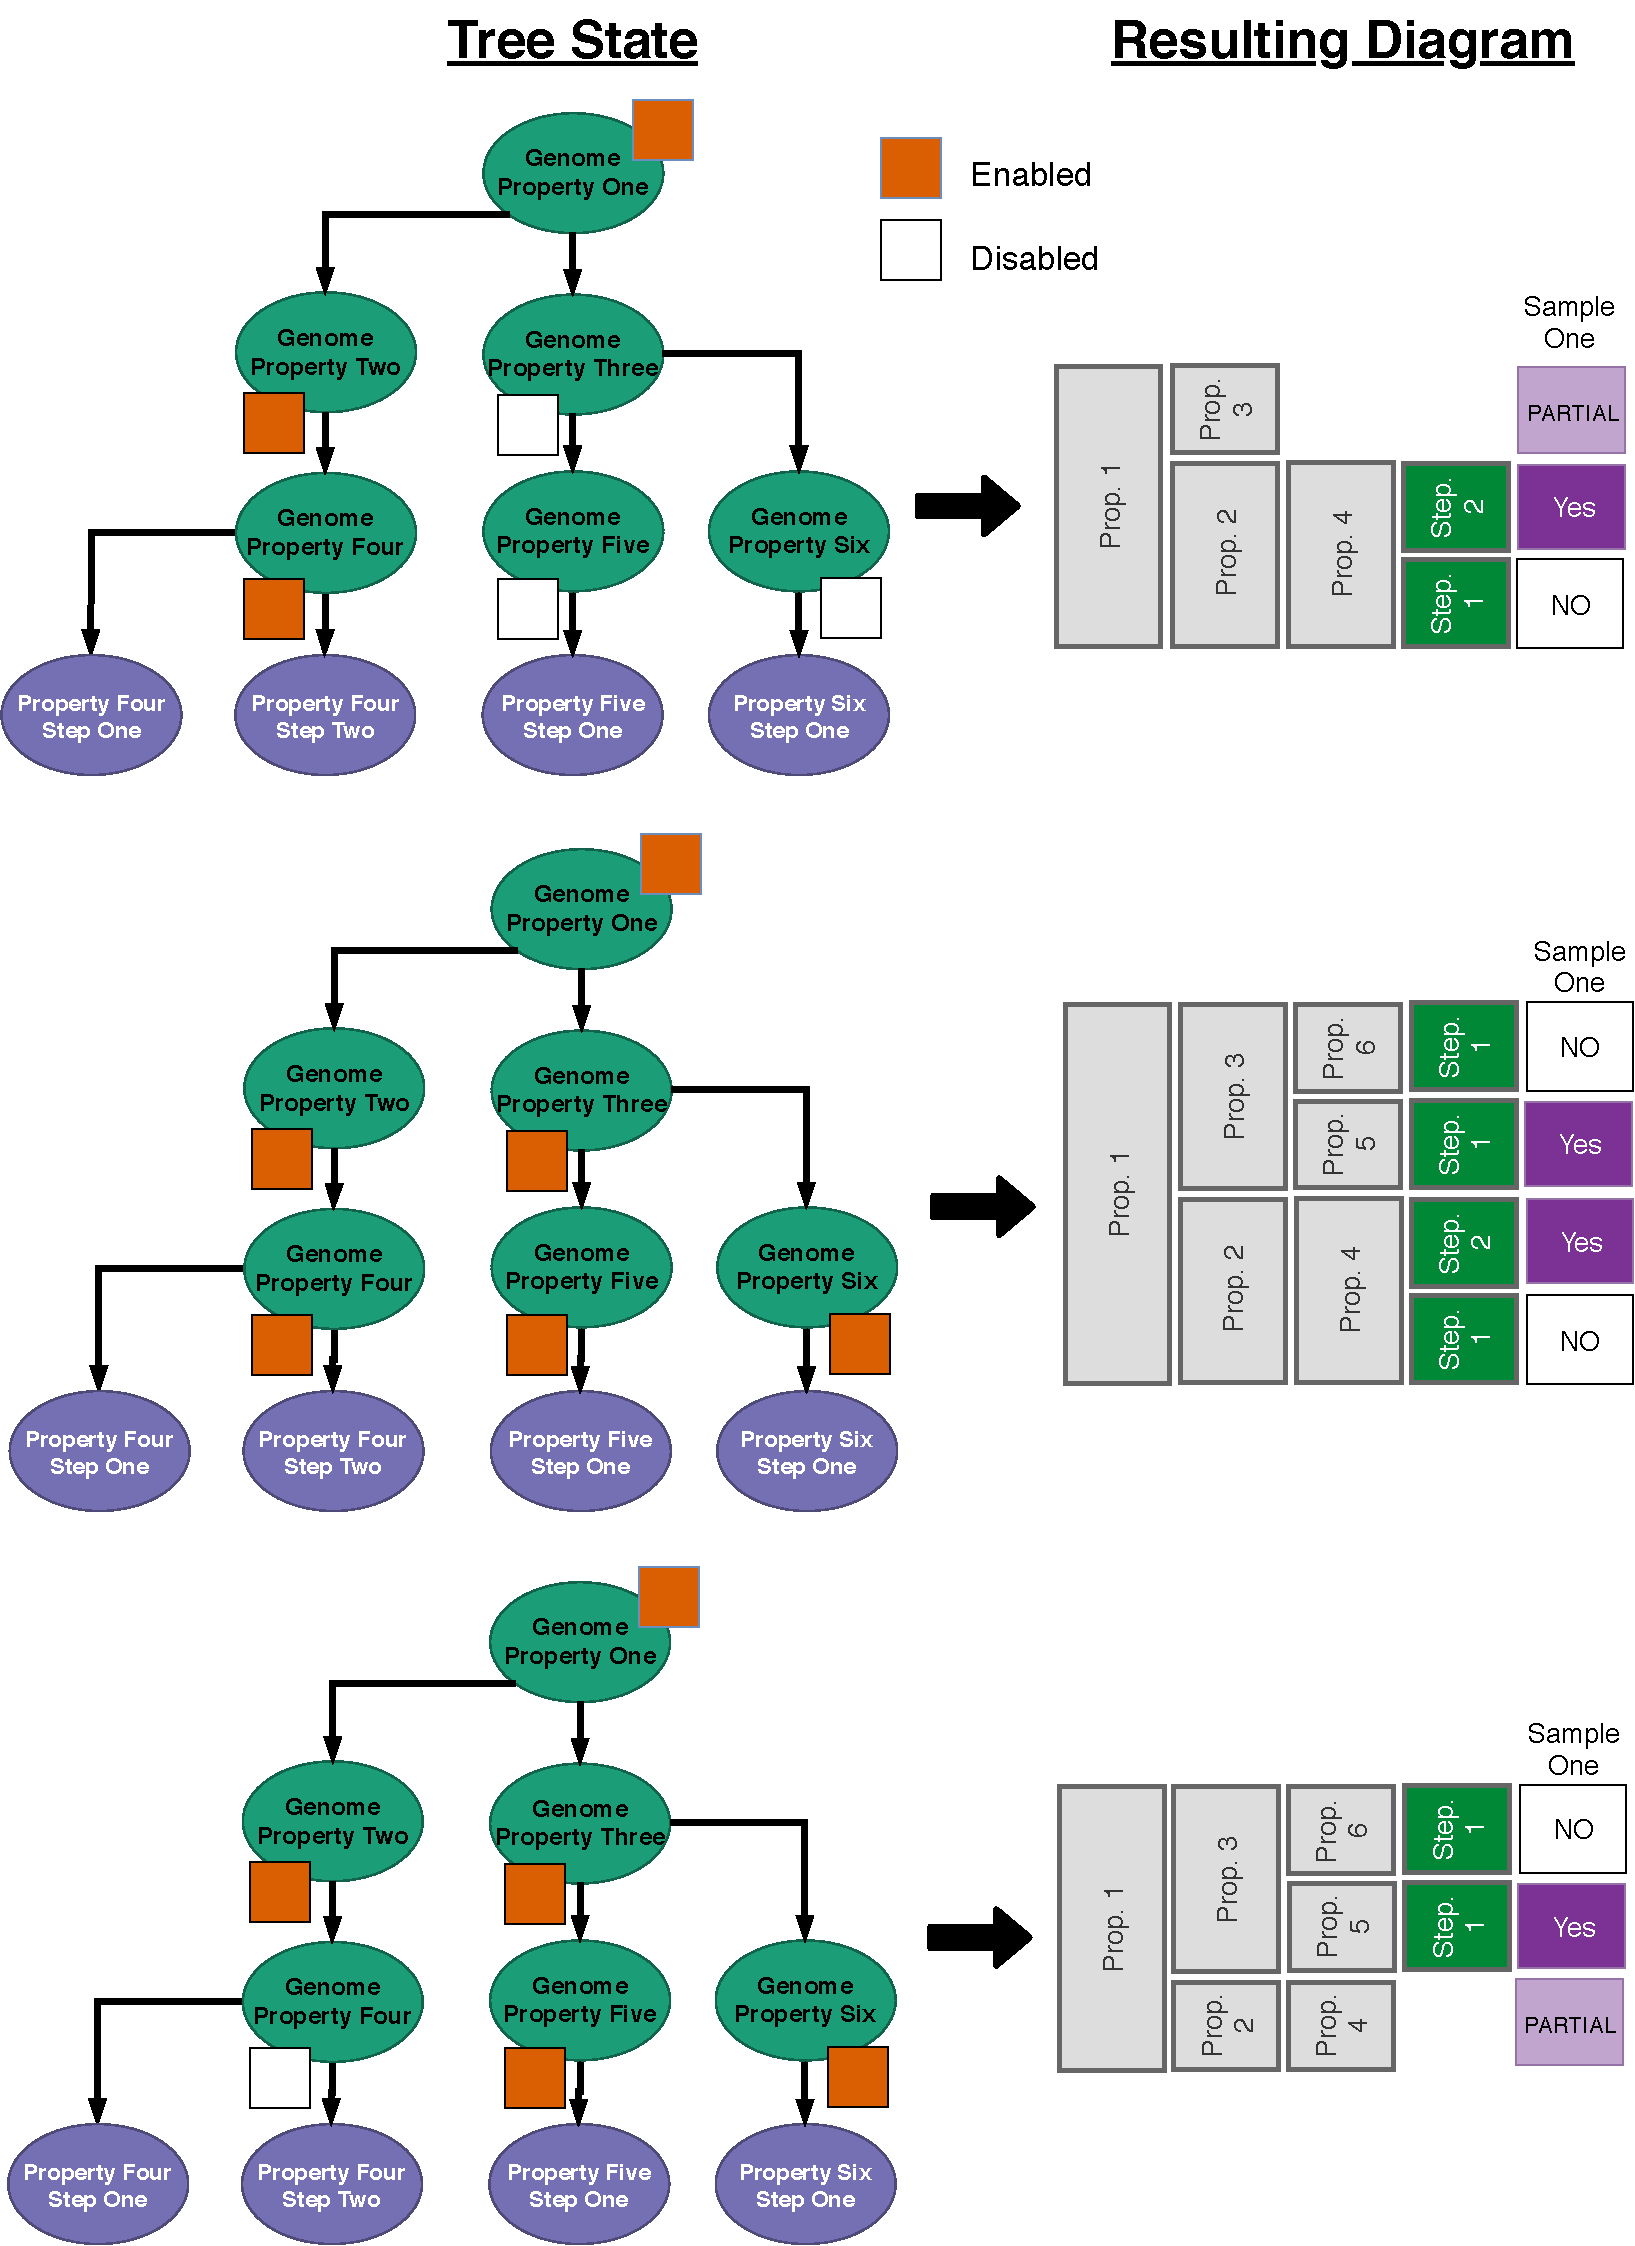
\includegraphics[width=0.7\textwidth]{media/how_tree_state_maps.pdf}
	 \caption[How the state of Micromeda-Client's heat map diagram is controlled by 
the state of a client-side in-memory property tree.]{\textbf{How the state of 
Micromeda-Client's heat map diagram is controlled by the state of a client-side 
in-memory property tree.} Changing the state of enabled attributes of property 
objects in the tree causes the heat map and icicle diagram to be generated 
differently on subsequent renderings. When a property is enabled, then its 
children are rendered in the heat map.}
	 \label{fig:tree-map-to-viz}
\end{figure}

\subsection{Loading the Visualization}

As mentioned previously, requests for data from Micromeda-Server supports much 
of the functionality of Micromeda-Client. All these requests are done through a 
technique known as \gls{ajax} \cite{garrett2005ajax,li2012jquery} (see 
\href{http://en.wikipedia.org/wiki/Ajax_(programming)}{en.wikipedia.org/wiki/ 
Ajax\_(programming)}). \gls{ajax} allows requests to be made to the server, 
using \gls{javascript} \cite{flanagan2006javascript}, without the need for a web 
page reload. This technique allows Micromeda-Client to remain asynchronous to 
the server where it was downloaded. \gls{ajax} requests are made via \gls{http} 
\cite{fielding1999hypertext}, through a series of \gls{url} addresses 
\cite{berners1994rfc} that map to Micromeda-Server endpoints (see Section 
\ref{endpoints}). All \gls{ajax} requests to the server were made using the 
JQuery \gls{javascript} library \cite{chaffer2013learning,li2012jquery}. The 
\gls{url} address of Micromeda-Server, where \gls{ajax} requests are made to, is 
found in a \gls{json} file called server\_config.json. This \gls{json} 
configuration file is deployed with the \gls{html} files of the client (i.e., 
the \gls{html} files for the client's visualization page and upload page). Both 
the file upload and visualization page call this \gls{json} file upon their 
initial load to acquire the location of Micromeda-Server.

The upload page contains a file drag and drop zone. When a user drops a 
Micromeda file onto this zone, the file is sent via \gls{ajax} to Micromeda-Server 
using the server's \textbf{upload} endpoint (Subsection \ref{endpoint-upload}). 
The drag and drop zone was implemented using DropzoneJS \cite{meno}. After the 
file upload is complete, Micromeda-Server returns the file's associated dataset 
key to Micromeda-Client. This dataset key is stored in the browser's web local 
storage \cite{Hickson} 
(\href{http://en.wikipedia.org/wiki/Web_storage}{en.wikipedia.org/wiki/Web\_storage}) 
using a library called localForage \cite{localforage}. Once the dataset key is 
stored, the client redirects the browser to the visualization page where 
visualizations of uploaded file's contents are generated.

As the visualisation page loads, the client requests a \gls{json} tree from 
Micromeda-Server's \textbf{get\_tree} endpoint (Subsection \ref{get-tree}) via 
\gls{ajax} . The dataset key saved in the browser's local storage is provided 
with this request and ensures that Micromeda-Server returns data from the 
browser's most recently uploaded Micromeda file. Micromeda-Server will respond 
to the \textbf{get\_tree} request by returning \gls{json} tree containing 
assignments for all properties and steps within this uploaded Micromeda file. 
The client parses this \gls{json} file into a \gls{javascript} object tree and 
uses it as the property tree data structure mentioned in Subsection 
\ref{visual-data-structures}. The visualization is then built using the 
dimensions from the diagram configuration array, the contents of the property 
tree and the \textbf{enabled} attribute of the property objects therein 
Subsection \ref{visual-data-structures}. The visualization itself is generated 
using functions from version 3.0 of the D3.js visualization library 
\cite{bostock2015d3} and custom \gls{javascript} code.

\subsection{Interactivity After Initial Visualization Load}

One of the critical properties of the client's visualizations is that they are 
interactive. This interactivity is provided by manipulating the \gls{javascript} 
property tree (Fig. \ref{fig:tree-map-to-viz}). When a user clicks a property 
node in the icicle diagram, a \gls{javascript} onclick event \cite{dom-events} 
(\href{http://en.wikipedia.org/wiki/DOM_events}{en.wikipedia.org/ 
wiki/DOM\_events}) is triggered that changes the state of the equivalent 
property object in the property tree data structure. Specifically, the clicked 
node's equivalent property object's \textbf{enabled} attribute is inverted upon 
icicle node click (Fig. \ref{fig:tree-map-to-viz}) and the entire visualization 
is subsequently re-rendered. Because the enable attribute has changed on the 
property object, the heat map visualization is re-rendered in a different 
configuration (Fig. \ref{fig:tree-map-to-viz}). 

In the case where a user clicks a leaf node of the icicle diagram, the client 
changes the matching property object's \textbf{enabled} attribute from false to 
true. Then, when the diagram is subsequently re-rendered, the children of the 
clicked node are also rendered (Fig. \ref{fig:tree-map-to-viz}). The client then 
scrolls the page so that the X-axis labels are aligned with the top of the 
clicked node. All scrolling behaviour in the client is facilitated by JQuery 
\cite{li2012jquery}. The opposite occurs when users click a non-leaf node of the 
icicle diagram. The client changes the associated property object's 
\textbf{enabled} attribute from true to false and, after re-rendering, the 
node's children are removed from the diagram. The client then scrolls so that 
the X-axis labels are aligned with the top of the clicked node. When a parent 
property object's \textbf{enabled} attribute is changed, this change is not 
cascaded to its children. This lack of transfer provides the visualization with 
a sort of ``memory" where the visibility state of each grandchild property is 
retained (Fig. \ref{fig:tree-map-to-viz}).

At page load, the property tree is used to create a \gls{javascript} array of 
pairs of property names and identifiers. After the visualization generation, an 
interactive search menu is created in the top right-hand corner of the 
Micromeda-Client interface (Fig. \ref{fig:micromeda-interface}). This menu is 
built using the Select2 library \cite{select2} 
(\href{http://select2.org}{select2.org}) and uses the previously mentioned pairs 
of property identifiers and names as search data. When a user searches for a 
property name or identifier in the search menu, properties whose name or 
identifier are similar to the search query are displayed in a drop-down menu 
(Fig. \ref{fig:micromeda-interface}). When the user clicks one of these menu 
properties, then another \gls{javascript} event occurs where the parent of the 
matching property object in the \gls{javascript} property tree is modified. All 
property objects along the property tree in a path from the root to the parent 
of matching property object have their \textbf{enabled} attribute set to true. 
When client visualization is subsequently re-rendered, a path to the assignments 
of the clicked property is displayed along with the property's assignments. The 
client software then automatically scrolls the page, via \gls{javascript}, so 
that the bottom of the X-axis labels are aligned with the top of the icicle 
diagram cell representing the clicked property.

After each re-rendering of the assignment visualization, Micromeda-Client sends 
a series of \gls{ajax}  requests to Micromeda-Server. These are requests for 
information about each property that is visible in the icicle diagram (Fig. 
\ref{fig:micromeda-interface}). These requests are sent to Micromeda-Server's 
\textbf{Get\_Single\_Genome\_Property \_Info} endpoint (Subsection 
\ref{get-property-info-endpoint}). The endpoint returns a \gls{json} document 
containing the information about each property that is later used in property 
information pop-up boxes (Fig. \ref{fig:micromeda-interface}). The contents of 
these documents are also cached in web local storage using localForage 
\cite{localforage}. During the subsequent diagram renderings, requests are not 
made for properties with data already cached. This caching reduces request 
frequency to the server and overall server load. The request volume is also 
reduced by only making requests for properties that are visible.

Both property information and \gls{fasta} download pop-up boxes are generated upon 
activation of \gls{javascript} onmouseover events \cite{dom-events} 
(\href{http://en.wikipedia.org/wiki/DOM_events}{en.wikipedia.org/wiki/DOM\_events}) 
of the question mark and step download glyphs, respectively. When a question 
mark glyph of a property icicle diagram node is hovered over, information about 
the property is retrieved from web local storage using localForage. This 
property information was cached during the previous diagram render. If no 
information for a property was previously cached, a template is used. The cached 
or template property information is used to generate the contents of the 
property information pop-up box. The \gls{fasta} download pop box, when generated, 
contains links for downloading \gls{fasta} files. These links point to \gls{url}s 
provided by Micromeda-Server's \textbf{get\_fasta} endpoint (Subsection 
\ref{get-fasta-endpoint}). When the``get all proteins" link is clicked (Fig. 
\ref{fig:micromeda-interface}), the endpoint \gls{url}'s \textbf{all} \gls{http} 
GET parameter is set to true during the request and a \gls{fasta} file containing all 
proteins that support the step is returned (see Subsection 
\ref{get-fasta-endpoint}). The \textbf{all} \gls{http} GET parameter is not 
added to requests initiated by clicking the ``get top proteins" link of the 
pop-up. This lack of a parameter causes the return of a \gls{fasta} file containing 
only the proteins that are most likely to support a step. During both of these 
types of requests, the dataset key stored in local web storage is attached. This 
key tells the Micromeda-Server to generate \gls{fasta} files from sequences found in 
the browser's most recently uploaded Micromeda file. Both pop-up boxes are hidden 
upon removal of the user's cursor via the triggering of an onmouseout event 
\cite{dom-events} 
(\href{http://en.wikipedia.org/wiki/DOM_events}{en.wikipedia.org/wiki/DOM\_events}).

\section{Interface Performance}

Performance testing found that the client's visualization was capable of being 
re-rendered almost instantaneously even when several hundred rows of assignments 
were displayed. All interactive components of Micromeda-Client had almost no 
visual lag attributed to their construction. All \gls{ui} lag was caused by 
waiting for data from Micromeda-Server endpoints. Ways of speeding up these 
endpoints are discussed in Section \ref{micromeda-server-improvements}.

\section{End-User Testing}

Three potential users of Micromeda-Client were provided with a visualization of 
data relevant to their research projects. These users were interviewed 
afterwards and their suggestions for improving the client's \gls{ui} were 
recorded. Several of their suggestions are discussed in Section 
\ref{client-improvements}. 

\section{Deployment}

Before Micromeda's \gls{ui} can be used, it must be downloaded into a web 
browser. A web server must be made available to send the client code to the 
user's browser. Micromeda-Client can be deployed in two ways. The client can be 
served from a web server, such as NGINX \cite{reese2008nginx}, running on the 
same server computer system as Micromeda-Server (Fig. 
\ref{fig:client-deployment}). Such a web server is already a component of the 
medium-scale deployment of Micromeda-Server described in Subsection 
\ref{single-server-micromeda-deployment}. Alternatively, Micromeda-Server can be 
served from a \gls{cdn} \cite{farber2003internet} 
(\href{http://en.wikipedia.org/wiki/Content_delivery_network}{en.wikipedia.org/wiki/Content\_delivery\_network}) 
such as Amazon Cloudfront \cite{varia2014overview} 
(\href{http://aws.amazon.com/cloudfront}{aws.amazon.com/cloudfront}) or 
Cloudflare Anycast \cite{calder2015analyzing} 
(\href{http://cloudflare.com/cdn}{cloudflare.com/cdn}). In this deployment 
configuration, the end-user downloads the client code from the nearest content 
delivery server in the \gls{cdn} , rather than the same server where 
Micromeda-Server is hosted (Fig. \ref{fig:client-deployment}). After loading, 
the client would then send \gls{api} requests to Micromeda-Server, which would 
be hosted outside the \gls{cdn}  (Fig. \ref{fig:client-deployment}). During 
end-user testing, a version of Micromeda-Client was deployed via Amazon 
Cloudfront \gls{cdn}. The files for Micromeda-Client could also be downloaded 
and opened by a developer's web browser for development and testing purposes.

\begin{figure}[!ht]
  \centering
	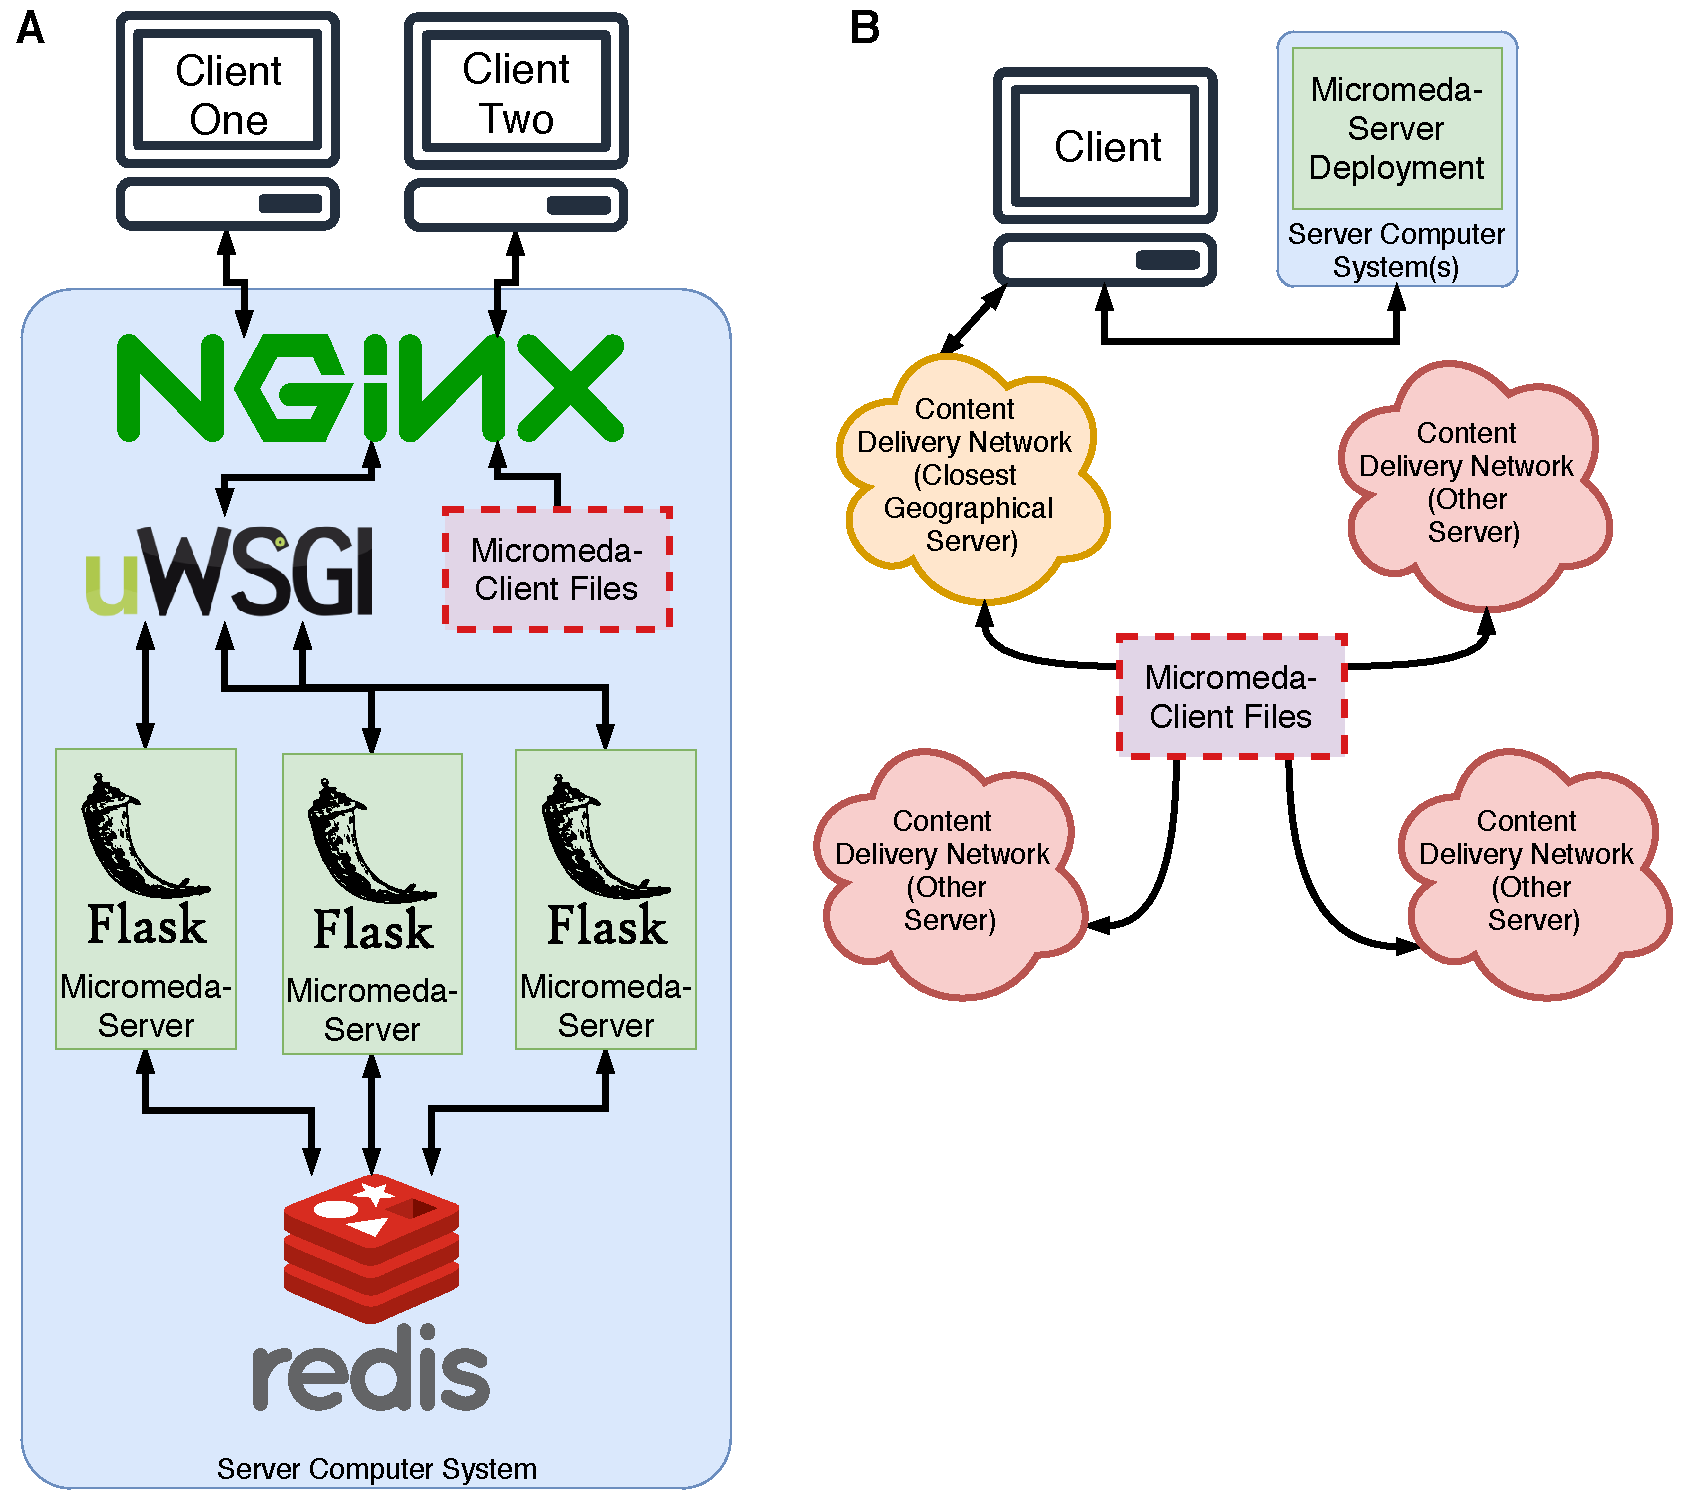
\includegraphics[width=0.7\textwidth]{media/micromeda-client-deployment.pdf}
	 \caption[The two primary deployment strategies for 
Micromeda-Client.]{\textbf{The two primary deployment strategies for 
Micromeda-Client.} The client files for Micromeda-Client, in production, can 
either be deployed on the same server computer system as Micromeda-Server (A) or 
deployed via a \gls{cdn} (B).}
	 \label{fig:client-deployment}
\end{figure}

\section{Future Improvements} \label{client-improvements}

Several improvements could be made to the client that would increase its overall 
usefulness. These features would make the client more natural to use and provide 
users with more information about their datasets. Several of these potential 
improvements were derived from feedback gathered during end-user testing.

\subsection{Providing More Information About Property Steps}

In the current version of Micromeda-Client, there are pop-up boxes that provide 
additional information about individual genome properties, such as property 
descriptions and links to equivalent records in other pathway databases. 
However, there are no equivalent pop-up boxes for providing more detailed 
information about property steps. The Genome Properties database includes 
additional information about steps that could be displayed in another set of 
pop-up boxes. For example, using information about what domains support a step 
could be used to generate links to domain records on the InterPro website. These 
links could be added to the suggested step pop-up boxes. Also, such pop-up boxes 
could provide \gls{go} terms and links to details about these terms on the 
\gls{go} website because individual steps are associated with such terms. The 
information in step information pop-up boxes would provide additional context to 
heat map step assignments. The boxes would be activated by hovering over a 
question mark glyph placed slightly above the download glyph of each step node 
in the client's icicle diagram (Fig. \ref{fig:micromeda-interface}). The 
addition of step information pop-up boxes would require an additional endpoint 
to be added to Micromeda-Server.

\subsection{Providing Improvements to Search Capability}

Currently, the search menu in the top right corner of the client interface 
allows users to search for genome properties by name or identifier (Section 
\ref{client-additional-features} and Fig. \ref{fig:micromeda-interface}). The 
ability to search for properties could be expanded by allowing users to search 
for properties by the identifier of equivalent records from \gls{kegg} 
\cite{kanehisa2000kegg} or MetaCyc \cite{karp2002metacyc}. These new search 
terms would allow users, who are familiar with the identifiers of specific 
\gls{kegg} or MetaCyc pathways, to rapidly find the equivalent pathway's genome 
property and its assignments in the Micromeda-Client heat map. It may also be 
useful to be able to search for property steps, rather than just properties, by 
name and have the visualization open a path and scroll to the assignment row for 
a searched step. Steps could also be searched for by their associated InterPro 
domain signature identifiers or \gls{go} term numbers. Improved ability to 
search for properties and steps would require additional endpoints to be added 
to Micromeda-Server.

\subsection{Automating the Scaling of the Visualization for Different Screen 
Sizes}

As mentioned in Subsection \ref{visual-data-structures}, the visualization 
generated by Micromeda-Client relies upon a file called 
\textbf{diagram\_configuration.json} that contains a series of measurements. 
These measurements consist of length, width, and spacing values that control the 
layout of the client's heat map and icicle diagram (Fig. 
\ref{fig:diagram-measurements}). The default values for these measurements, as 
stored in \textbf{diagram\_configuration.json}, facilitate the generation of an 
adequate diagram layout for most datasets. However, for several datasets, such 
as those with long organism names or large numbers of samples, the default 
diagram measurements can cause visual anomalies such as text clipping between 
diagram cells and organism names being displayed off-page.

To fix such anomalies, future versions of Micromeda-Client could use 
\gls{javascript} to automatically adjust diagram configuration measurements to 
fit different datasets or different window sizes better. For example, X-axis 
spacing values could be changed dynamically based on the length of the longest 
organism name in a dataset. Alternatively, the heat map cell width could be 
adjusted based on the number of samples in a dataset. By adjusting the default 
diagram layout values dynamically, Micromeda-Client could generate diagrams that 
better fit a variety of datasets and user devices.

\subsection{Modification of Micromeda-Client to Collect Assignment Data From a 
Separate Endpoint}

Currently, Micromeda-Client gathers its assignment data from the 
\textbf{get\_tree} endpoint of Micromeda-Server (Subsection \ref{get-tree}). 
There are problems with this approach, as discussed in Subsection 
\ref{assignment-endpoints}, and it would be more appropriate to have a separate 
server endpoint for returning assignments for properties and steps. In addition 
to solving the problems mentioned, having the client make a separate \gls{api} 
call to gather these assignment data would be useful as it would allow the client 
to request for Micromeda-Server to rearrange the data before it is returned. 
This reconfigurability would also allow for step assignments that are supported 
by protein domains to be replaced by match \gls{eval} scores or for assignments 
of organisms to be returned in a different order.

\subsection{Clustering Heat Map Columns by Assignment Similarity}

Columns in the heat map contain assignments from different organisms. Currently, 
these columns are ordered alphanumerically by organism name. Users may find it 
useful to be able to cluster these columns by assignment contents rather than by 
name. Clustering by assignment contents would group organisms that have similar 
assignments and potentially similar metabolic, physiological, or structural 
characteristics. Columns could be clustered either globally by the assignments 
of all properties and steps or locally by only those properties and steps that 
are visible in the current diagram rendering. The simplest solution for 
clustering these columns would be to use Micromeda-Server. As noted in 
Subsection \ref{assignment-endpoints}, if the return of property and step 
assignments were pushed to a separate endpoint, then the data returned would 
have to be generated by serializing assignment DataFrames of 
GenomePropertiesResultsWithMatches objects to \gls{json} \cite{bray2014rfc}. If 
clustering columns in the heat map was required, then Micromeda-Server could 
accomplish this visual clustering by clustering the DataFrames of 
GenomePropertiesResultsWithMatches objects column-wise using \gls{scikit}-learn 
\cite{pedregosa2011scikit} using pandas. Afterwards, these clustered DataFrames 
would then be converted to \gls{json} and sent to the client. Returning 
clustered assignment \gls{json} data could be controlled by an \gls{http} GET 
parameter in an endpoint request.

\subsection{Visualizing Step Assignments by E-value Score Rather Than by 
Categorical Assignment} \label{interface-e-value}

Leaf genome properties are supported by steps that use InterProScan matches to 
InterPro consortium domain signatures as evidence. These matches, between a 
motif found in a protein of an organism and an InterPro domain, have an 
\gls{eval} score. Micromeda-files store these scores. Matches with \gls{eval} 
scores that are below a specific per-InterPro member database threshold are 
filtered out by InterProScan automatically. Matches that remain are likely to be 
true positives (\textit{i}.\textit{e}., the motif matched is an ortholog to the domain from the 
database). However, there is still some \gls{eval} score variation among the 
remaining matches. Motifs with matches that have lower \gls{eval} scores are 
closer in sequence to domains in the database and are more likely to be 
orthologous. These lowest \gls{eval} matches are be said to be the``strongest" 
matches.

During end-user testing, several potential users were interested in having a way 
to compare the relative strength of step assignments between organisms. For 
example, if a property is assigned YES in two organisms, which organism is more 
likely to possess a step? Step assignments are currently assigned a binary YES 
or NO, and thus the relative strength of these assignments cannot be compared. 
One way to compare step assignments between organisms would be to compare the 
strength of these assignments' supporting domain matches. For example, 
Micromeda-Client could display the \gls{eval} score of the closest match 
supporting each step in its heat map in place of a binary YES or NO value. These 
\gls{eval} scores could be coloured by shades of green along a continuous scale. 
Pop-up boxes could also be generated by hovering over each cell in the heat map 
cell and would display match info, such as the \gls{eval} score, protein name, 
and matched domain identifier. No \gls{eval} data would be presented for NO 
assignments. An interface switch could be implemented that would be used to 
switch property assignments between binary YES or NO values and continuous 
\gls{eval} scores. A Micromeda-Server endpoint would have to be built to provide 
these \gls{eval} score data, as discussed in Subsection \ref{e-value-endpoint}.

\subsection{Improving Filtering Capability of the Client}

A \gls{ui} switch would have to be implemented that would allow users to switch 
between a complete assignment view of all assignment rows and only those that 
differ. The assignment rows would have to be dropped based on those that are 
displayed in the current version of the heat map. Each node in the 
\gls{javascript} property tree could be given a property called 
\textbf{differing} that returns true if the property's associated assignments 
are differing between organisms and false otherwise. Children of nodes on the 
\gls{javascript} property tree whose state is set to \textbf{enabled} would only 
be rendered if their \textbf{differing} property is set to true.

The icicle diagram could be re-rooted based on the assignments and child 
assignments of a specific property. For example, having the visualization show 
the property for iron metabolism and its children. This feature could be 
implemented by having a glyph on each node of the icicle diagram that, when 
clicked, allows for the diagram to be re-rooted at the node. In the future, this 
feature could be expanded for users to select multiple properties to display, 
for example by clicking three of the re-root glyphs and an interface button. Being 
able to perform selections in this way would allow users only to compare the 
assignments of two or more properties that are distant in the Genome Properties 
\gls{dag}.

\section{A Comparison of Micromeda-Client to Other Pathway Visualization 
Software} \label{visualization-comparison}

Several web-based software tools already exist for visually comparing the 
presence and absence of biochemical pathways across organisms. However, while 
interviewing potential users of Micromeda-Client, the interviewees conveyed 
their frustration with these existing tools. Users mentioned how these tools 
forced them to navigate through multiple web pages to gather the information 
needed to perform their analyses. This process is time-consuming and 
error-prone. In response to this information, Micromeda-Client was designed to 
integrate as much information as possible into a single view and interactivity 
is used to show and hide information as needed by users. Below is a detailed 
comparison between Micromeda-Client and three similar visualization tools.

As of fall 2019, there is only one Genome Properties assignment visualization 
tool available other than Micromeda-Client. This tool is part of the \gls{ebi} 
Genome Properties website \cite{richardson2018genome} 
(\href{http://www.ebi.ac.uk/interpro/genomeproperties}{ebi.ac.uk/interpro/genomeproperties}) 
and has an assignment viewing page that displays a heat map similar to the one 
generated by Micromeda-Client \cite{richardson2018genome} (Fig. 
\ref{fig:property-viewer} and see 
\href{http://www.ebi.ac.uk/interpro/genomeproperties/#viewer}{ebi.ac.uk/interpro/genomeproperties/\#viewer}). 
In contrast to Micromeda-Client, information about the properties displayed is 
not accessible from the heat map itself and must be viewed in a secondary web 
page. This page contains a property browser (Fig. \ref{fig:property-browser} and 
see 
\href{http://www.ebi.ac.uk/interpro/genomeproperties/#browse}{ebi.ac.uk/interpro/genomeproperties/\#browse}). 
Even when a user finds a property on this browsing page, they must open a third 
page that contains the property's information such as a description and links to 
equivalent records. Thus, with the Genome Properties website, if users need a 
more detailed description of a property, then they are forced to swap between 
multiple web pages. To effectively use the \gls{ebi} tool, from a \gls{ui} 
perspective, users should place both property browser and assignment viewer 
windows side by side. However, using both of these windows simultaneously 
requires either a large monitor or two monitors placed side by side because the 
assignment heat map page of the website does not scale down well with a 
shrinking window size. If both property information and assignment information 
pages are open simultaneously on a 14" laptop, then the controls of the 
assignment heat map page are cut off, and the visualization becomes unusable. 
Unlike Micromeda-Client, the Genome Properties website's assignment viewer only 
displays a subset of leaf genome properties and their steps, not all properties 
and steps (Fig. \ref{fig:property-viewer}). The website also does not perform 
any aggregation of assignments to reduce the length of its heat map (Fig. 
\ref{fig:property-viewer}). Like the client, users can upload their data. In the 
case of the \gls{ebi} assignment viewer, users can upload InterProScan \gls{tsv} 
files instead of Micromeda files \cite{richardson2018genome}. Thus, there is no 
way for users to access the underlying protein sequences that support each step.

In contrast to the property assignment heat map generated by the Genome 
Properties website, Micromeda-Client uses pop-up boxes to display its property 
information. Users of Micromeda-Client do not have to search for the property 
that they are interested in an entirely new window, nor do they need to swap 
between multiple windows. Having all the information in a single view saves 
users time and reduces mistakes where users view information about the wrong 
property. Also, unlike the \gls{ebi} Genome Properties website, Micromeda-Client 
displays assignments for all properties, not just leaf properties. The icicle 
diagram that is present in the client's visualization helps organize property 
assignments, so users more easily find these assignments. Unlike the \gls{ebi} tool, the 
client's assignment viewer does use interactive aggregation and disaggregation, 
which decreases the length of its heat maps substantially.

\begin{figure}[!ht]
   \centering
   \begin{subfigure}[b]{0.46\textwidth}
     \centering
     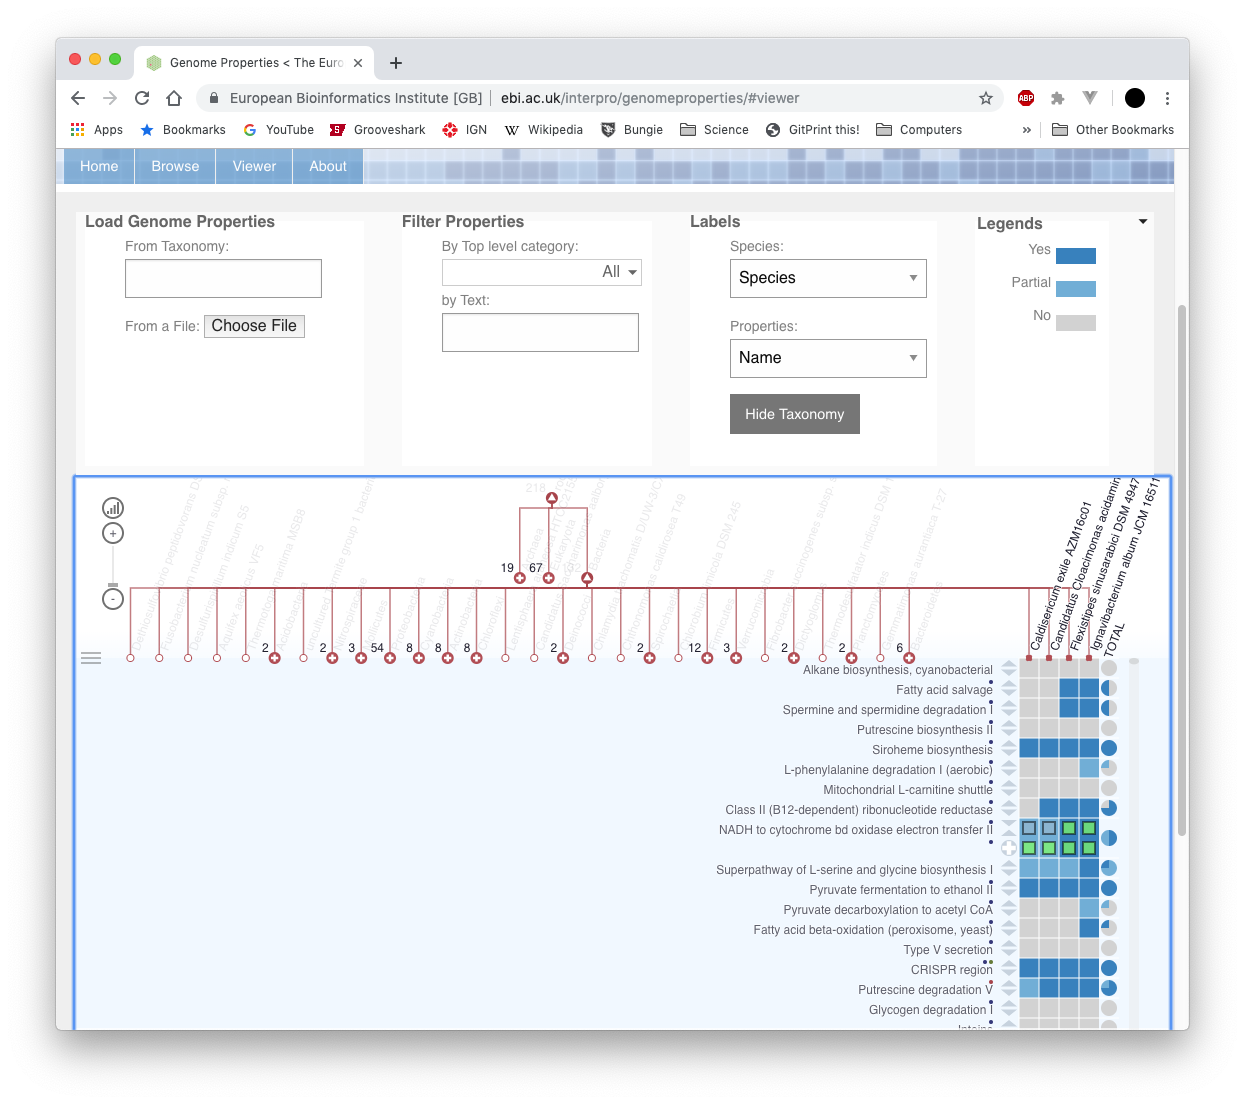
\includegraphics[width=\textwidth]{media/genome_properties_viewer.png}
     \caption{The Genome Properties viewer displays heat maps containing 
assignments for both reference and novel organisms.}
     \label{fig:property-viewer}
   \end{subfigure}
   \qquad % some horizontal space
   \begin{subfigure}[b]{0.46\textwidth}
     \centering
     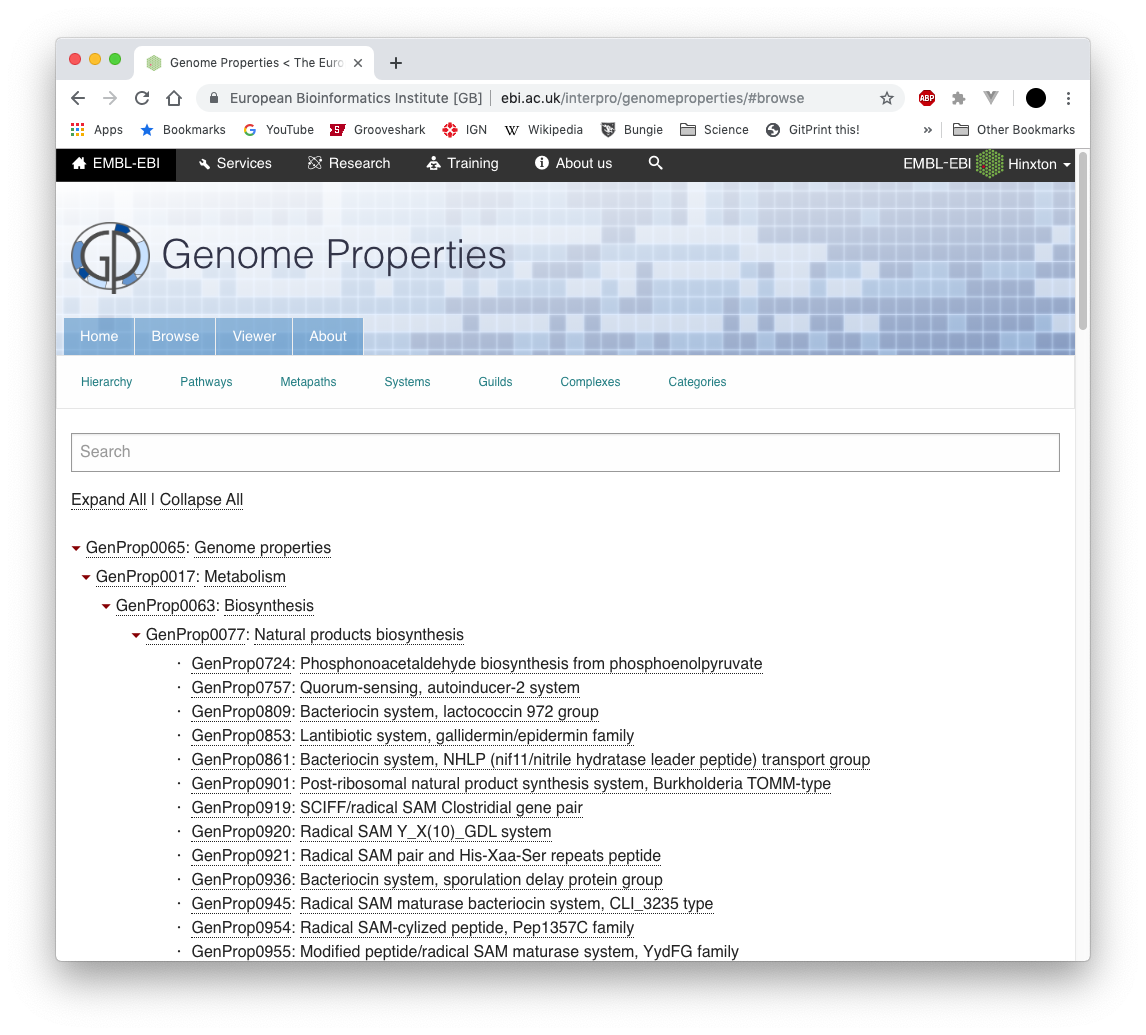
\includegraphics[width=\textwidth]{media/genome_properties_browser.png}
     \caption{The Genome Properties browser provides information about 
individual properties and their hierarchy.}
     \label{fig:property-browser}
   \end{subfigure}
   \caption[Browser windows containing the two main webpages of the Genome 
Properties website.]{\textbf{Browser windows containing the two main webpages of 
the Genome Properties website.} The viewer page (a) is used for viewing property and 
step assignments. The browser page (b) helps users learn more about 
individual genome properties. The viewer page (a) allows for the upload of 
InterProScan \gls{tsv} files of novel organisms. These files are used to 
calculate assignments for these organisms. With Micromeda-Client, the same 
information presented by these two pages is integrated into a single page.}
   \label{fig:genome-properties-interface}
\end{figure}

Other websites that visualize pathway annotation information do use aggregation 
and disaggregation in the same way as Micromeda-Client 
\cite{vallenet2016microscope,darzi2019functree2}. However, some of these tools 
have interface issues. For example, Microscope \cite{vallenet2016microscope}, a 
pathway annotation website, also presents heat maps conveying levels of 
completeness for \gls{kegg} \cite{kanehisa2000kegg}, MetaCyc 
\cite{karp2002metacyc}, and \gls{antismash} \cite{blin2019antismash} pathways 
(Fig. \ref{fig:microscope}). Like the Genome Properties database, both 
\gls{kegg} and MetaCyc organize their pathways hierarchically. However, with 
Microscope, when a user clicks the visualization interface to gain access to the 
completeness of child pathways, an entirely new heat map is generated on a 
separate page. Child pathway assignments are not displayed within the same 
heat map view (Fig. \ref{fig:microscope}). When navigating results from 
high-level pathways to low-level pathways, users are required to open several 
heat map pages. To access a heat map containing results for pathway steps, 
users may have to open five or more separate pages. In addition to opening each 
level of the visualization on a separate page, if users need to find additional 
information about a pathway, then they need to click on links that take them to 
a separate page. This page mirrors a page on the \gls{kegg} or MetaCyc website 
that describes the pathway (Fig. \ref{fig:microscope}). There is no way to 
compare the cousin pathway results within the same heat map 
(Fig. \ref{fig:microscope}).

\begin{figure}[!ht]
 \centering
	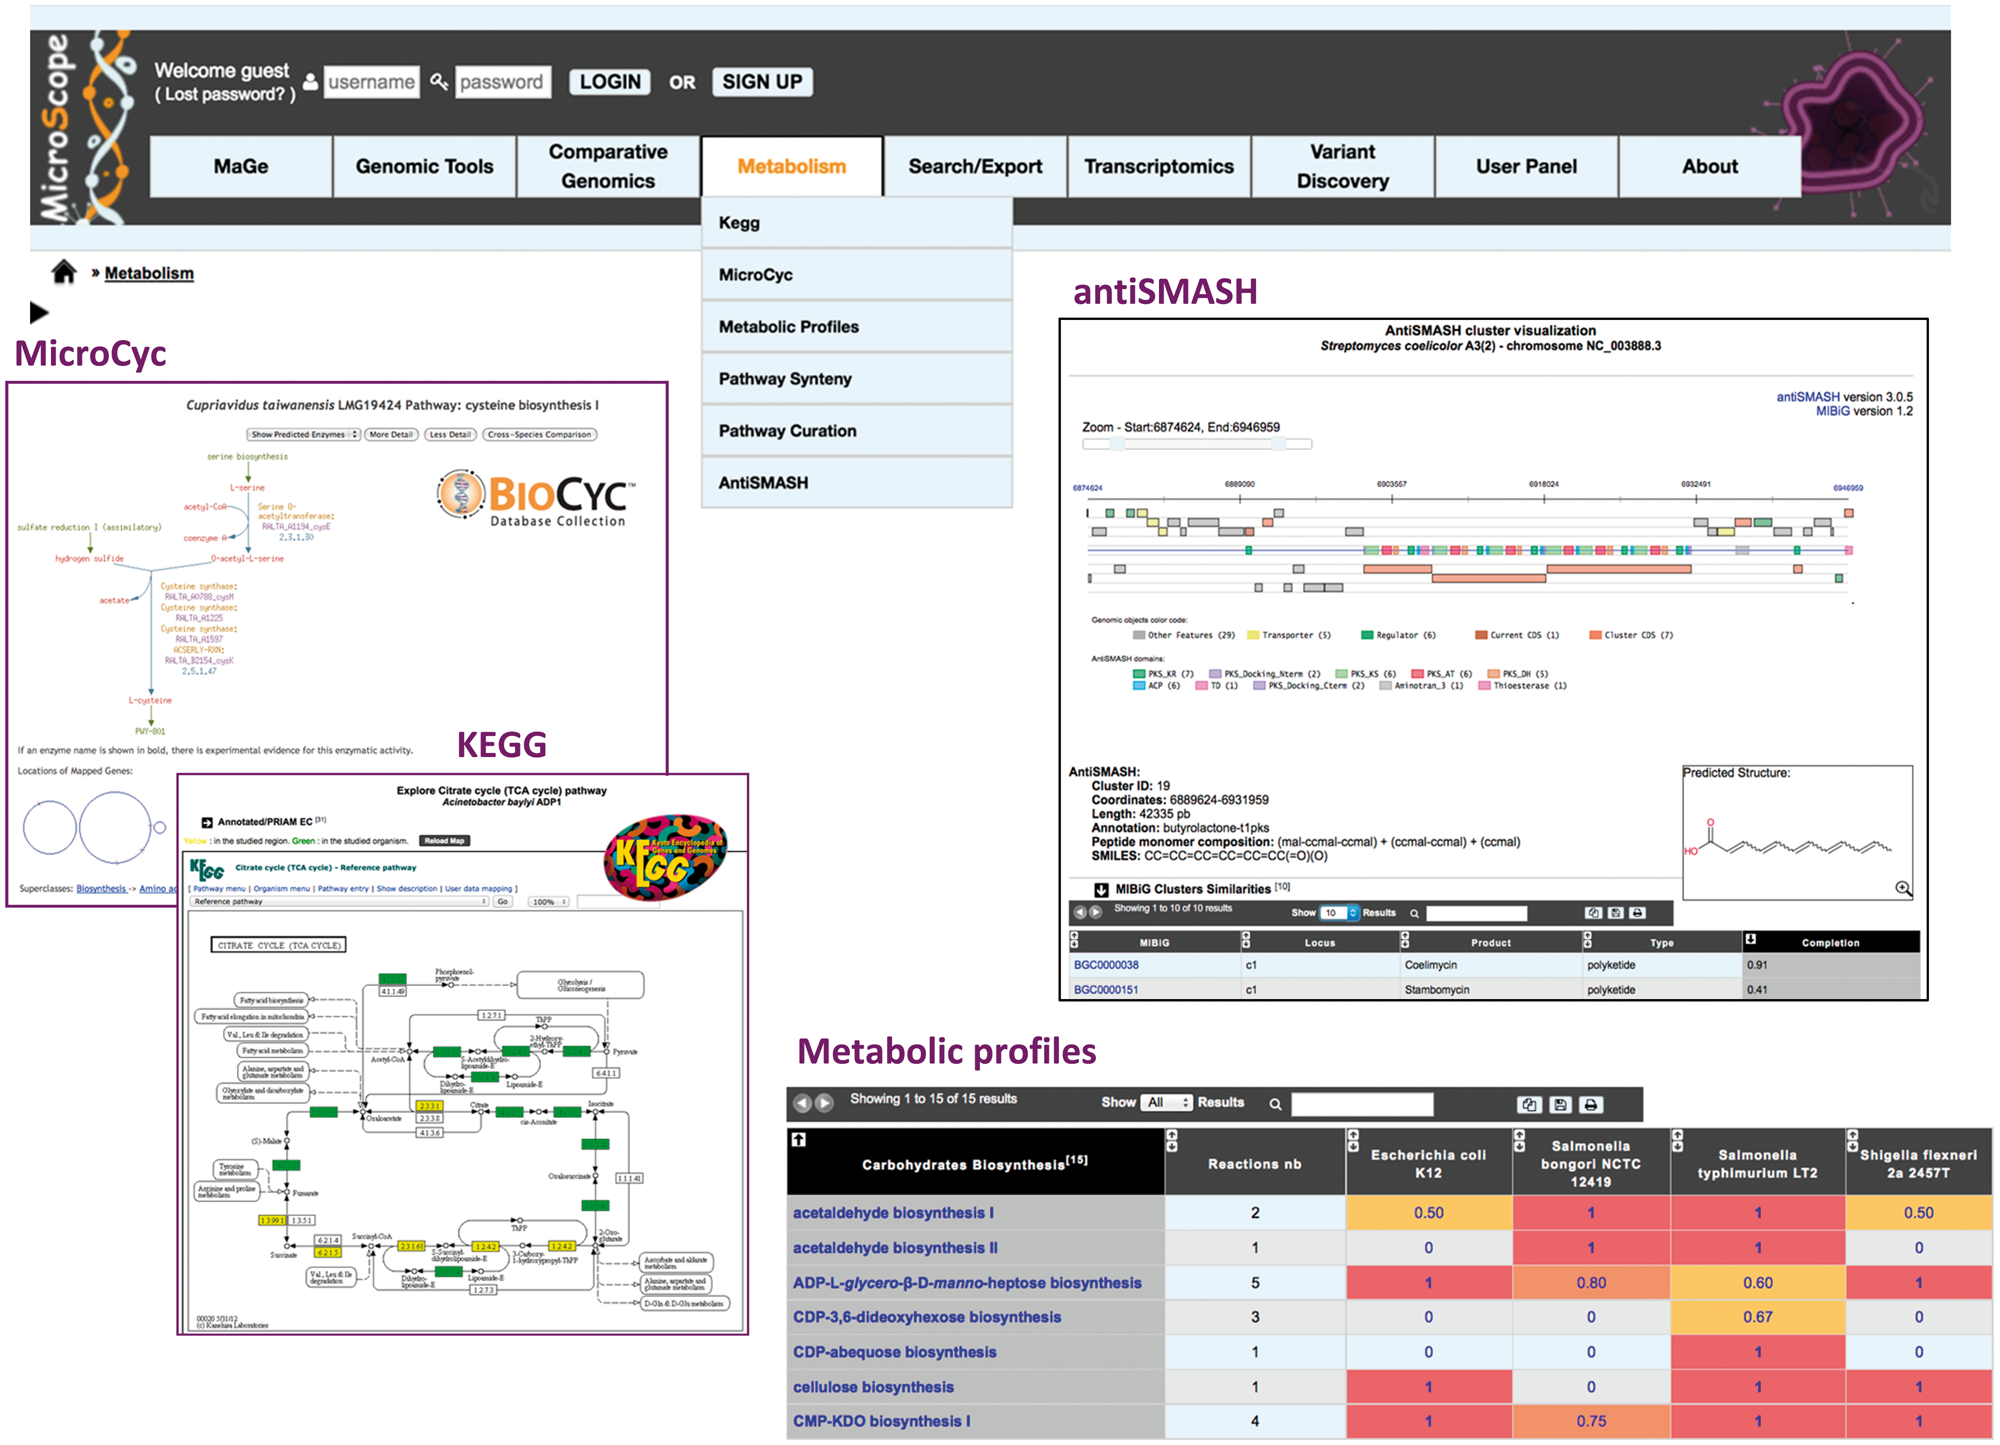
\includegraphics[width=0.9\textwidth]{media/microscope.png}
	 \caption[User interface of and analysis services provided by the MicroScope 
annotation server.]{\textbf{User interface of and analysis services provided by 
the MicroScope annotation server.} The server presents both pathway assignment 
heat maps and pathway diagrams. The heat maps show the presence and absence of 
pathways across reference organisms and novel organisms whose genomes have been 
uploaded in \gls{fasta} format. The pathway diagrams allow users to explore 
further the pathways annotated by the server. Figure is from 
\cite{vallenet2016microscope}.}
	 \label{fig:microscope}
\end{figure}

In contrast to Microscope, Micromeda-Client displays its aggregated and 
disaggregated heat map rows within the same view. Thus, users are not required 
to swap back and forth through multiple pages to find child pathway results and 
to understand how results for parent properties are calculated. Information 
about the properties is also accessible through pop-ups from within the same 
view. The assignment of cousin properties is easily seen within the same heat 
map view.

\begin{figure}[!ht]
 \centering
	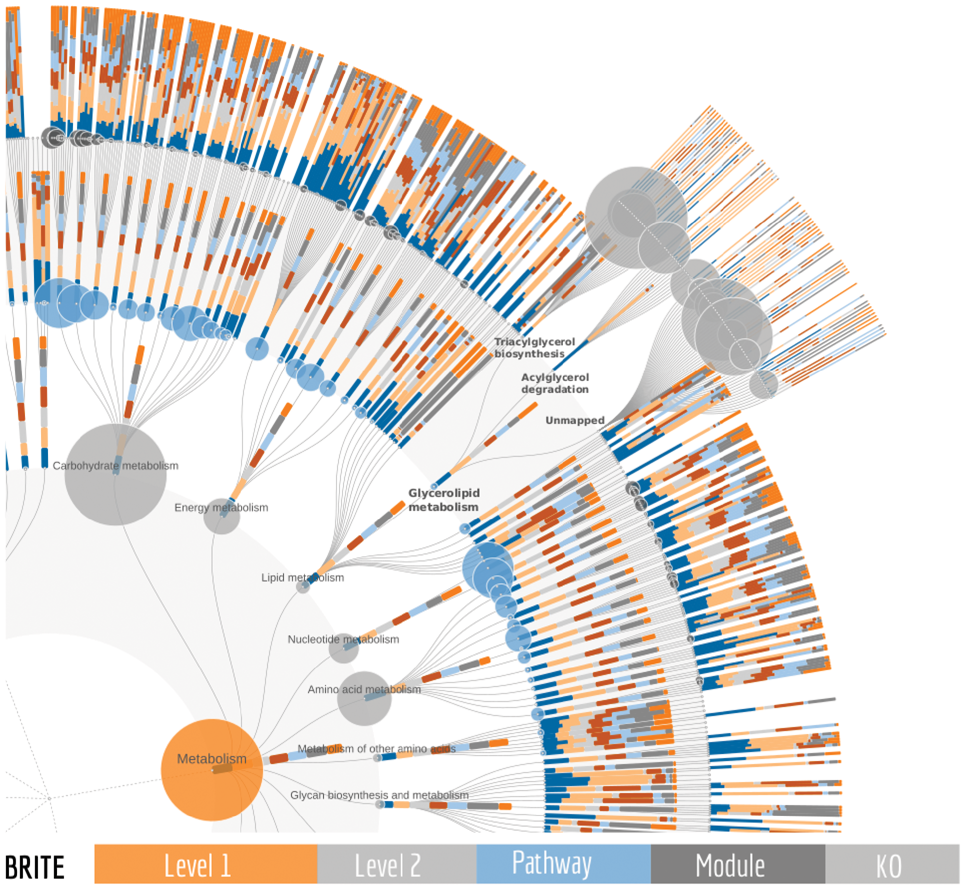
\includegraphics[width=0.7\textwidth]{media/functree2.png}
	 \caption[Overview of the KEGG annotation visualization produced by 
FuncTree2.]{\textbf{Overview of the \gls{kegg} annotation visualization produced 
by FuncTree2.} FuncTree2 presents a radial tree diagram that shows the abundance 
of \gls{ko} annotations within multiple organisms' predicted proteomes. In 
diagrams created by the tool, leaves of the radial tree represent individual 
\gls{ko} annotations. In other words, each leaf node represents a type of 
protein that can be found in a cell. Nodes closer to the root represent 
different levels of classification that group these \gls{ko} annotations 
according to the hierarchy of pathways in the \gls{kegg} database. A stacked bar 
chart annotates each leaf node. This chart possesses coloured bars representing 
the number of proteins in each organism's proteome with a specific \gls{ko} 
annotation. These bar charts are oriented radially. Stacked Bar charts also 
annotate other nodes in the radial tree. The stacked bar charts on higher-level 
nodes represent reciprocal summations of \gls{ko} counts of child nodes. Nodes 
can be clicked to remove child nodes and change the shape and size of the 
visualization. Figure is from \cite{darzi2019functree2}.}
	 \label{fig:functree2}
\end{figure}

In contrast to the Genome Properties website and Microscope, some alternative 
annotation visualization tools do present their data hierarchically within the 
same visualization \cite{darzi2019functree2}. For example, FuncTree2 
\cite{darzi2019functree2} allows users to plot \gls{ko} annotation 
\cite{mao2005automated,kanehisa2011kegg} frequency (i.e, the number of proteins 
of an organism that that possess a specific \gls{ko} annotation) across 
multiple organisms (Fig. \ref{fig:functree2}). Frequencies are visualized using 
a radial tree with nodes annotated by stacked bar charts. The bar charts of leaf 
nodes of the tree represent counts for a singular \gls{ko}, whereas charts 
annotating nodes closer to root display summed \gls{ko} counts for child nodes 
(Fig. \ref{fig:functree2}). Unlike Micromeda-Client, aggregated and 
disaggregated data are presented simultaneously. Nodes in the tree can be clicked 
to add and remove child nodes from the visualization. Instead of a default 
\gls{kegg}-based tree, users can also upload their tree and annotation frequency 
information.

One of the key design differences between FuncTree2 and Micromeda-Client is 
their choice of radial and linear layouts, respectively. In the application note 
for FuncTree2, its authors note that they chose to use a radial tree over 
horizontal trees in their visualization to save screen space. Radial trees are 
more space-efficient than horizontal trees when presenting large numbers of 
nodes \cite{burch2011evaluation}. However, at least one study has shown, via 
eye-tracking, that radial trees underperform traditional and orthogonal tree 
layouts for a variety of visual search tasks \cite{burch2011evaluation}. Another 
study has shown that icicle diagrams (as used by Micromeda-Client) allowed users 
to have higher interaction accuracy and efficiency \cite{muramalla2017radial} 
than radial sunburst diagrams (as used by tools such as Krona 
\cite{ondov2011interactive} 
(\href{http://github.com/marbl/Krona}{github.com/marbl/Krona}).
Such gains in user interaction capability should also carry over to 
Micromeda-Client, which uses a rectangular, rather than a radial 
layout\footnote{I assert that radial layouts are most useful when they show 
connections between data on opposite sides of the circle. This design pattern is 
used by visualization tools such as Circos \cite{krzywinski2009circos}.}.

Rather than defaulting to a horizontal tree or radial tree, micromeda's client 
replaces both of these trees with an icicle diagram. This icicle diagram 
provides superior spacial compactness to either tree type as no edges have to be 
rendered and nodes can be placed adjacently. Rectangular diagrams have better 
space utilization than radial diagrams on modern computer monitors 
\cite{muramalla2017radial}. In contrast to FuncTree2, the visualization of 
Micromeda-Client only allows users to show either aggregated assignments for a 
parent node or the disaggregated assignments of its children, not both 
simultaneously. Both the decision to use icicle diagrams and to either present 
parent or child assignments allow the client's diagram to retain the same square 
layout as an annotated horizontal tree with superior space utilization to a 
radial tree. 

\section{Summary} \label{micromeda-client-summary}

The web client of Micromeda allows users to visually explore and compare 
assignments for genome properties and their steps across organisms. The software 
also provides information about these properties and steps and provides links 
between them and equivalent records in other databases. Due to the use of 
Micromeda files, the client also allows users to download protein sequences that 
support the displayed assignments. These functionalities directly support the 
required tasks listed in Section \ref{visualization-design}.

As discussed in the Section \ref{visualization-comparison}, the client's 
visualization addresses many interface issues that afflict other pathway 
annotation visualization software tools. As discussed in the summary section of 
Chapter \ref{micromeda-server}, another feature that sets Micromeda apart from 
these tools is the access to supporting information used in property and 
step assignments such as protein sequences. In the future, and as discussed in 
Subsection \ref{interface-e-value}, the data presented by Micromeda-Client could 
be further expanded to display more information such as E-value scores. 
Annotation frequency, as displayed by default by FuncTree2, could also be 
readily displayed by the client. Overall, Micromeda-Client will increase users' 
ability to utilize pathway annotation information and set a new standard for 
pathway annotation visualizations.
